\documentclass[letterpaper,journal]{IEEEtran}
\usepackage{amsmath,amsfonts}
\usepackage{algorithmic}
\usepackage{algorithm}
\usepackage{array}
\usepackage[caption=false,font=normalsize,labelfont=sf,textfont=sf]{subfig}
\usepackage{textcomp}
\usepackage{stfloats}
\usepackage{url}
\usepackage{verbatim}
\usepackage{graphicx}
\usepackage{cite}
\usepackage{tabularx}
\usepackage{booktabs}
\hyphenation{op-tical net-works semi-conduc-tor IEEE-Xplore}
% updated with editorial comments 8/9/2021

\begin{document}

\title{Optical Integrated Sensing and Communication for 6G: A Cross-Modality Survey and Metric-Governed Roadmap}

\author{Fatih D\"onmez, Ahmet Altuncu, and Mustafa Namdar,~\IEEEmembership{Member, IEEE}%
    \thanks{Fatih D\"onmez and Ahmet Altuncu are with the Department of Electrical and Electronics Engineering, Afyon Kocatepe University, Afyonkarahisar, Turkiye (e-mail: fatih.donmez@usr.aku.edu.tr; aaltuncu@aku.edu.tr). Fatih D\"onmez ORCID: 0000-0003-0553-4418. Corresponding author: Fatih D\"onmez.}%
    \thanks{Mustafa Namdar is with the Department of Electrical and Electronics Engineering, Faculty of Engineering, Kutahya Dumlupinar University, Kutahya, Turkiye (e-mail: mustafa.namdar@dpu.edu.tr).}}

\markboth{Draft Manuscript}%
{D\"onmez \MakeLowercase{\textit{et al.}}: Optical Integrated Sensing and Communication Review}

\maketitle

\begin{abstract}
    Optical Integrated Sensing and Communication (O-ISAC) is emerging as a 6G design direction because optical carriers can support high-rate links and sensing functions across guided fiber, free-space optical, VLC/LiFi, and photonics-assisted high-frequency platforms. Yet the literature remains fragmented by modality, terminology, measurement plane, and metric semantics, making direct comparison risky without an explicit governance layer.

    This systematic review synthesizes 220 peer-reviewed O-ISAC studies using a PRISMA-grounded process and develops a cross-modality taxonomy spanning medium class, integration mechanism, detection/observability regime, and sensing task. We introduce a metric-governed reporting contract that separates bandwidth-limited range resolution $\Delta r_{\min}$, estimator-level accuracy such as $\sigma_r$/RMSE, CRB/FIM bound statements, fiber spatial granularity $\Delta z$, and optical/electrical signal-quality planes. This contract enables conservative rate--resolution analysis and capacity-resolution quotient (CRQ) synthesis only when rate and sensing metrics are reported under compatible scenario records.

    The review further maps enabling technologies, including optical RIS/ORIS, optical phased arrays, photonic integration, photonics-assisted mmWave/THz generation, and ML/security-aware adaptation, and links them to deployment constraints and benchmark needs. The resulting roadmap identifies the reporting practice, taxonomy alignment, reproducible evaluation workflows, scalable hardware, and domain-aware validation needed for credible O-ISAC progress.
\end{abstract}

\begin{IEEEkeywords}
    Optical integrated sensing and communication, O-ISAC, free-space optics, visible light communication, distributed fiber sensing, photonic-terahertz systems, systematic review.
\end{IEEEkeywords}



\section{Introduction}
\label{introduction}

Integrated sensing and communication (ISAC) has become a central 6G theme because future networks are expected to exchange data, infer geometry, localize users and objects, monitor infrastructure, and adapt to environmental context within the same operating fabric \cite{O_ISAC_070,O_ISAC_162}. Optical integrated sensing and communication (O-ISAC) extends this joint-service idea into optical carriers, guided fiber links, free-space optical links, visible-light/LiFi deployments, and photonics-assisted mmWave/THz chains \cite{O_ISAC_021,O_ISAC_068,O_ISAC_303}. This move is not simply RF-ISAC at a higher carrier frequency. Optical systems expose much larger nominal spectral resources, strong spatial directionality, and mature photonic multiplexing, but they also introduce medium-specific constraints: fiber is guided and often monitored through distributed sensing granularity, FSO is weather- and pointing-sensitive, VLC/LiFi is intensity-domain and illumination-constrained, and photonic-THz systems couple optical generation/distribution to high-frequency wireless propagation \cite{O_ISAC_006,O_ISAC_023,O_ISAC_039,O_ISAC_070}.

The attraction of the optical domain is visible in representative demonstrations. Photonic-THz and fiber-wireless systems report very high data rates together with ranging or radar-style sensing, while multicore and coherent fiber studies show that communication capacity and distributed monitoring can coexist in guided infrastructure \cite{O_ISAC_016,O_ISAC_029,O_ISAC_043,O_ISAC_044,O_ISAC_046,O_ISAC_105}. VLC and LiFi studies, in contrast, often couple indoor data access with positioning, gesture, occupancy, or pose estimation through direct-detection and lighting-aware channels \cite{O_ISAC_009,O_ISAC_022,O_ISAC_039,O_ISAC_050,O_ISAC_062}. These examples motivate O-ISAC as a family of architectures rather than a single pooled performance category.

\begin{figure*}[!t]
    \centering
    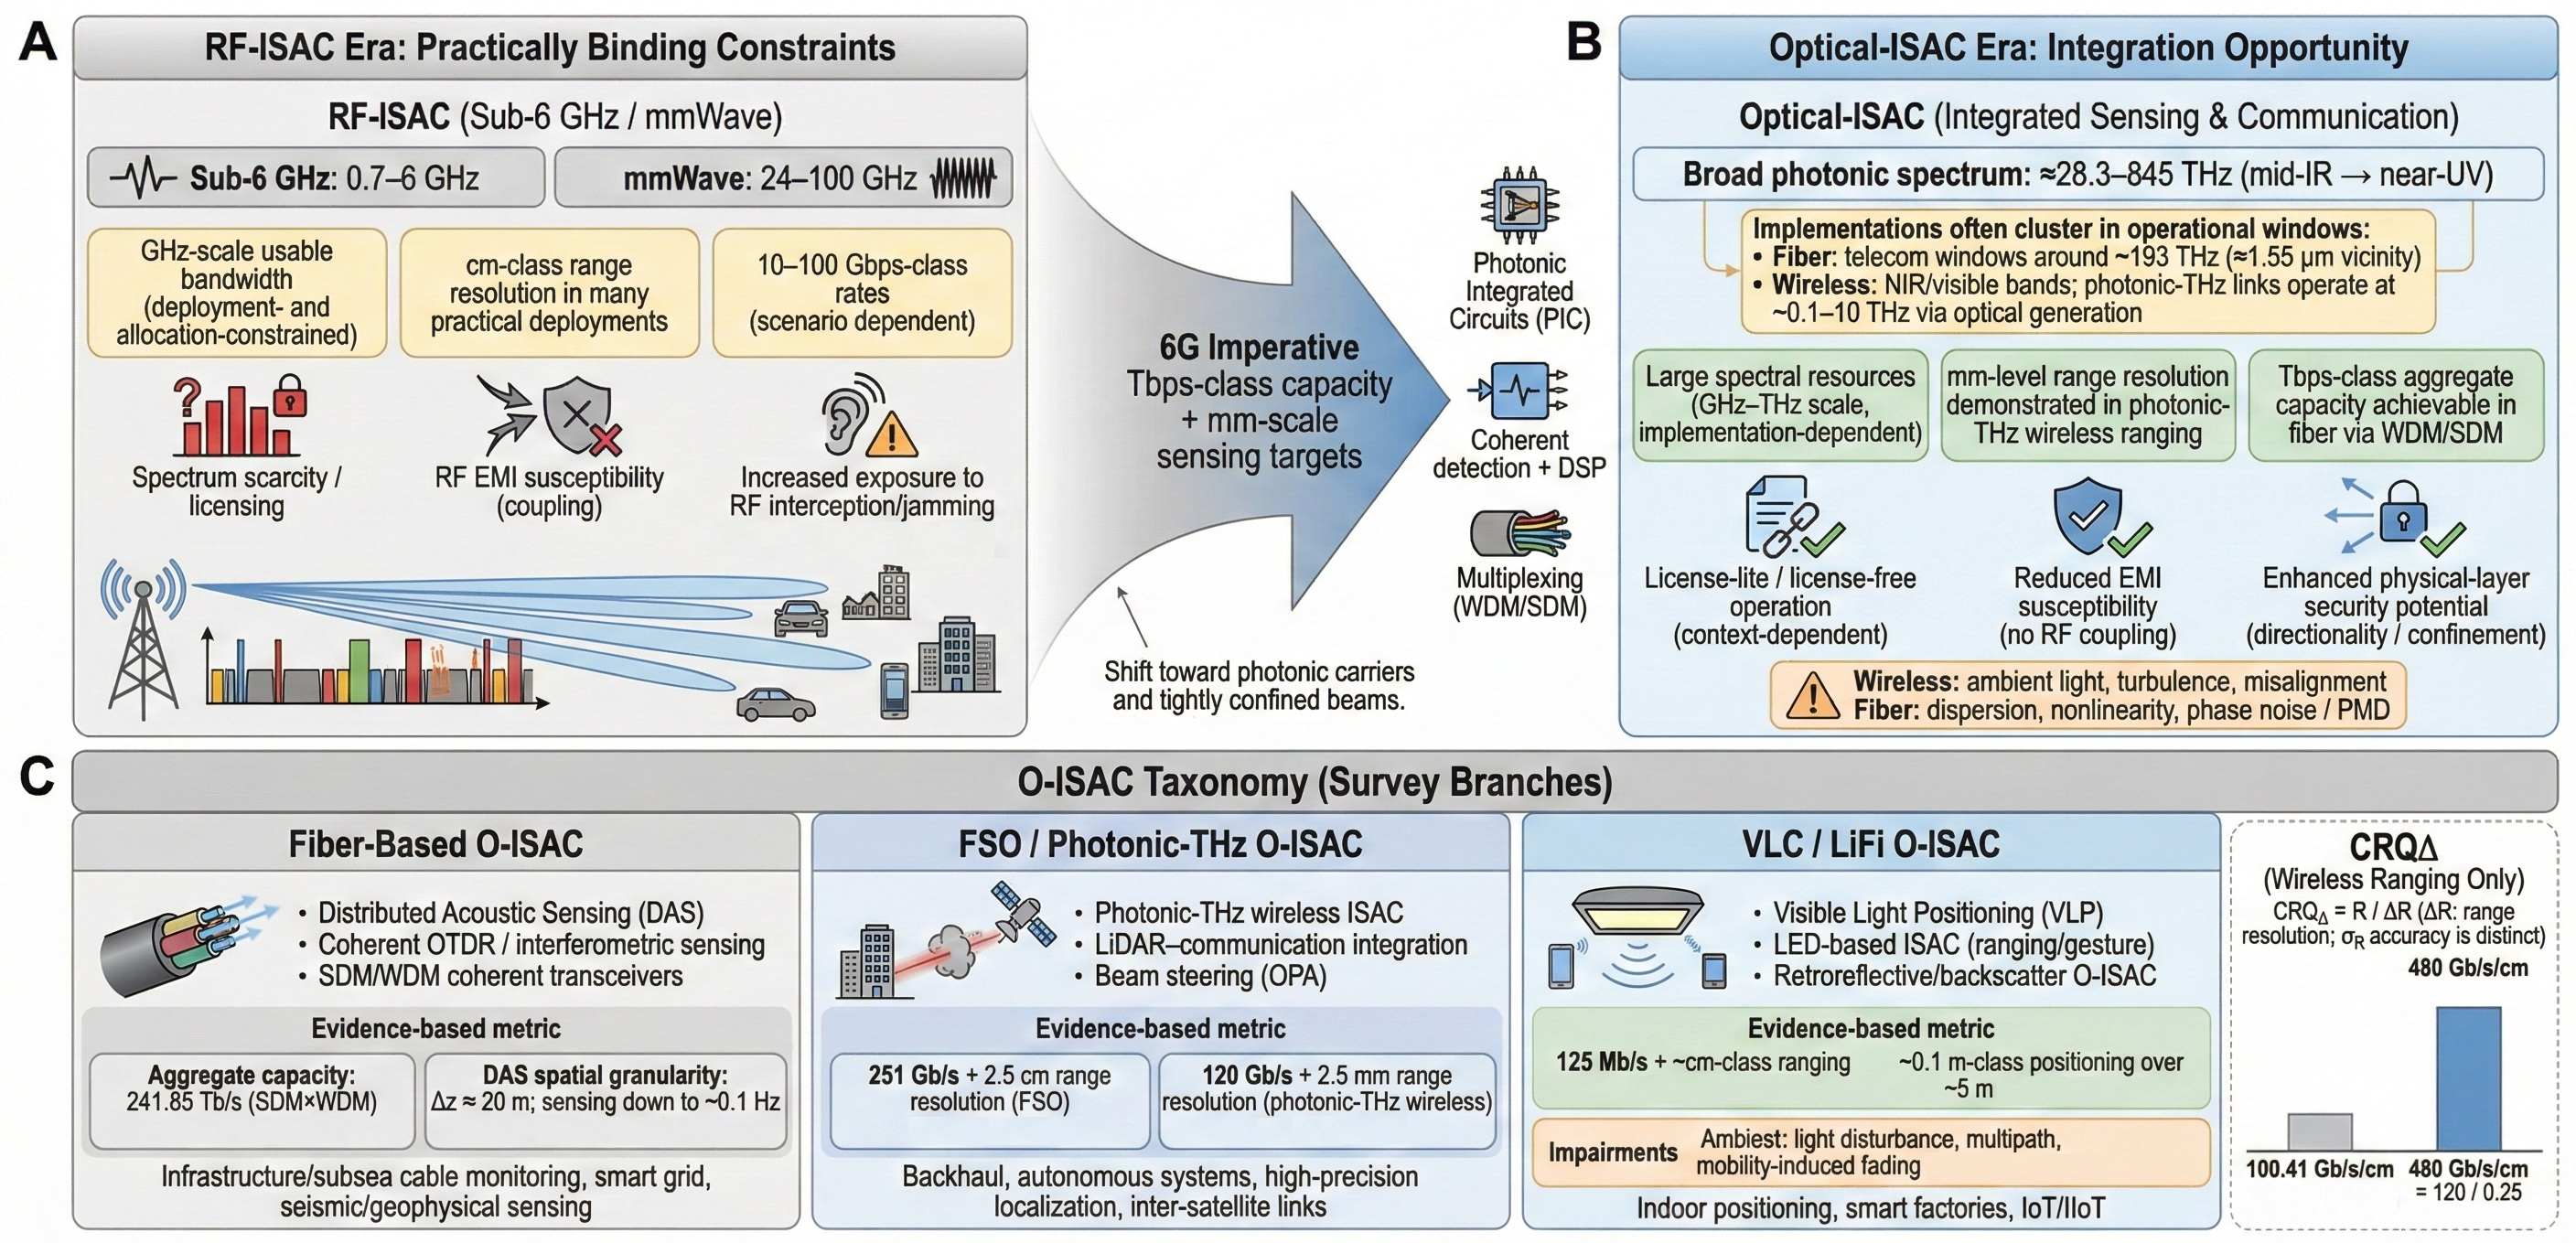
\includegraphics[width=\linewidth]{figures/fig1.jpg}
    \caption{O-ISAC landscape across optical spectrum resources and the main fiber, FSO/photonic-THz, and VLC/LiFi branches.}
    \label{fig:fig1}
\end{figure*}

Fig.~\ref{fig:fig1} provides the opening landscape. It separates the broad optical resource argument from the cross-modality synthesis problem. Wide optical bandwidth can support high-rate and fine-delay measurements, yet a fiber \(\Delta z\), a wireless \(\Delta r_{\min}\), an estimator RMSE, a CRB/FIM bound, an optical OSNR value, and an electrical SNR value are not interchangeable evidence objects. This review is built around that distinction. Instead of ranking papers by headline rate or sensing number, it asks when cross-paper comparison is admissible and which reporting fields are needed to make such comparison defensible.

The related survey landscape remains fragmented. RF-ISAC surveys and standardization-oriented discussions establish the broader 6G context but do not resolve optical-plane measurement issues \cite{O_ISAC_161,O_ISAC_162}. VLC/VLP surveys explain visible-light positioning and indoor optical channels, yet usually remain single-modality \cite{O_ISAC_068,O_ISAC_303,O_ISAC_327}. Fiber-oriented reviews emphasize distributed fiber-optic sensing, cabled infrastructure, or optical communication coexistence rather than cross-modality optical ISAC \cite{O_ISAC_006,O_ISAC_041,O_ISAC_090}. Photonic-THz and fiber-wireless reviews highlight high-frequency generation and integrated waveforms but do not fully bridge fiber, FSO, VLC/LiFi, and hybrid platforms under one metric contract \cite{O_ISAC_021,O_ISAC_035,O_ISAC_058,O_ISAC_070}. Table~\ref{tab:axis_comparison} summarizes the gap.

\begin{table*}[!t]
    \caption{Related survey landscape and the contribution of this review.}
    \label{tab:axis_comparison}
    \centering
    \scriptsize
    \setlength{\tabcolsep}{2.4pt}
    \renewcommand{\arraystretch}{1.08}
    \begin{tabularx}{\textwidth}{@{}p{1.25cm}p{0.58cm}p{1.55cm}Xc c c c c@{}}
        \toprule
        Work & Year & Scope & Main emphasis & Syst. & Cross-med. & Tax. & Metric gov. & CRQ \\
        \midrule
        \cite{O_ISAC_161} & 2025 & RF/6G ISAC & RF-centric survey framing and standardization context & No & No & Part & No & No \\
        \cite{O_ISAC_068} & 2024 & VLC & Visible-light JCS prospects and indoor positioning links & No & No & Part & No & No \\
        \cite{O_ISAC_327} & 2024 & VLC/VLP & VLC/VLP channel and localization survey & No & No & Part & No & No \\
        \cite{O_ISAC_006} & 2024 & Fiber & Fiber-sensing ISAC challenges & No & No & Part & No & No \\
        \cite{O_ISAC_021} & 2024 & Optical ISAC & Architecture, potential, and challenge tutorial & No & Part & Part & Part & No \\
        \cite{O_ISAC_070} & 2026 & Photonic THz & Photonic THz-ISAC waveform/system view & No & Part & Part & No & Part \\
        \cite{O_ISAC_163} & 2025 & RIS/ISAC & RIS-enabled ISAC enabler context & No & No & Part & Part & No \\
        This review & 2026 & All optical & PRISMA $N=220$, taxonomy, metric contract, governed tradeoff, enablers, applications, roadmap & Yes & Yes & Yes & Yes & Yes \\
        \bottomrule
    \end{tabularx}
\end{table*}

Four fragmentation mechanisms motivate the review. First, terminology is unstable: optical papers use O-ISAC, LiSAC, optical JCS, photonic ISAC, fiber-ISAC, fiber sensing/communication coexistence, and THz-over-fiber labels for overlapping ideas \cite{O_ISAC_021,O_ISAC_033,O_ISAC_041,O_ISAC_053,O_ISAC_068}. Second, the dominant metrics are not isomorphic across modalities. Third, the communities cite and benchmark within separate silos even when waveforms, calibration, or receiver concepts might transfer \cite{O_ISAC_042,O_ISAC_074,O_ISAC_080,O_ISAC_097,O_ISAC_113}. Fourth, application studies often show domain-specific feasibility without stating which evidence can generalize to other optical media \cite{O_ISAC_084,O_ISAC_123,O_ISAC_129,O_ISAC_143,O_ISAC_155,O_ISAC_160}.

This review contributes five items. First, it builds a PRISMA/TQAF evidence base over \(N=220\) peer-reviewed studies. Second, it defines a cross-modality taxonomy covering fiber, FSO, VLC/LiFi, photonic-THz, and hybrid platforms. Third, it introduces a metric-governance contract that separates \(\Delta r_{\min}\), \(\sigma_r\)/RMSE, CRB/FIM, \(\Delta z\), and OSNR/SNR/ESNR planes. Fourth, it performs a governed rate--resolution and CRQ synthesis that shows the CRQ-valid subset is sparse. Fifth, it links enablers, applications, and open challenges into a roadmap for reproducible, modality-aware O-ISAC research.

\subsection{Why Optical O-ISAC Needs Its Own Survey Layer}

The need for a dedicated O-ISAC survey follows from the fact that optical systems change both the useful resource and the failure mode. In RF-ISAC, the dominant constraints are typically spectrum availability, aperture size, waveform sharing, interference management, and regulatory coexistence. Optical systems inherit some of these concerns, but they also introduce wavelength-selective components, photodetection, optical/electrical conversion, beam pointing, eye-safety and illumination constraints, fiber dispersion and nonlinearities, and very different receiver observability regimes. A visible-light positioning paper and a coherent fiber sensing paper may both be O-ISAC, but they do not report the same physical layer. The same is true for a photonic-THz system in which optics generate or distribute a high-frequency carrier before wireless propagation occurs. For this reason, the review treats O-ISAC as a cross-modality family whose members need common reporting fields but not a single common channel model.

This stance also affects how prior surveys are used. Related surveys provide valuable modality anchors, such as VLC/VLP positioning, distributed fiber sensing, RF-ISAC standardization, RIS-enabled ISAC, and photonic-THz waveform discussions. They do not, however, provide a systematic evidence base that simultaneously compares fiber, FSO, VLC/LiFi, photonic-THz, and hybrid optical platforms under a metric contract. The resulting gap is not merely bibliographic. Without a common taxonomy and metric-governed reading, a reader can easily misinterpret a fiber spatial granularity as wireless range resolution, a CRB as measured accuracy, an OSNR value as electrical SNR, or an unmatched rate and sensing value as a valid CRQ point.

\subsection{How the Review Is Organized}

The paper therefore proceeds from physical and metric foundations to evidence synthesis. Section~\ref{sec:background_metric_contract} defines the receiver-plane and metric-governance contract. Section~\ref{sec:methodology} explains the PRISMA/TQAF evidence base and why a structured synthesis is more appropriate than a statistical meta-analysis. Section~\ref{sec:taxonomy} develops the cross-modality taxonomy. Section~\ref{sec:tradeoff} applies the metric contract to the rate--resolution and rate--accuracy evidence, preserving the sparse governed subset result. The final sections interpret enablers, deployment motifs, and roadmap challenges through the same governance lens rather than as isolated lists of technologies.

\section{Background and Metric-Governance Contract}
\label{sec:background_metric_contract}

An O-ISAC system can be represented as a source, modulation and waveform resources, a propagation medium, receiver observables, and communication/sensing estimators. This abstraction is useful only if the receiver and propagation planes remain explicit. Coherent optical receivers preserve complex-field information and therefore support phase-sensitive observability, carrier recovery, and optical-plane signal-quality measures. IM/DD receivers expose intensity-domain observations after photodetection, so their noise, SNR, and estimator behavior are normally electrical-plane quantities \cite{O_ISAC_001,O_ISAC_022,O_ISAC_028,O_ISAC_029,O_ISAC_039,O_ISAC_132}. Treating these observation modes as equivalent would erase a primary source of metric mismatch.

\begin{figure*}[!t]
    \centering
    
\includegraphics[width=\linewidth]{figures/fig_ii_1.png}
    \caption{Unified O-ISAC source--channel--observation abstraction with modality-specific propagation and receiver planes retained.}
    \label{fig:fig_ii_1}
\end{figure*}

Fig.~\ref{fig:fig_ii_1} summarizes the common chain while retaining modality-specific branches. In guided fiber, the signal propagates through a dispersive and nonlinear medium, and sensing often emerges through distributed fiber-optic sensing, vibration monitoring, strain, temperature, or co-route infrastructure monitoring \cite{O_ISAC_006,O_ISAC_013,O_ISAC_024,O_ISAC_032,O_ISAC_046,O_ISAC_076}. In FSO, atmospheric loss, turbulence, pointing, and geometry shape both rate and ranging behavior \cite{O_ISAC_005,O_ISAC_023,O_ISAC_035,O_ISAC_048}. In VLC/LiFi, Lambertian emission, LoS/NLoS composition, illumination constraints, and direct detection dominate the receiver-level model \cite{O_ISAC_009,O_ISAC_022,O_ISAC_039,O_ISAC_054}. In photonic-THz or hybrid systems, optical carriers may generate, distribute, or coherently receive high-frequency signals while wireless propagation occurs at mmWave/THz bands \cite{O_ISAC_026,O_ISAC_029,O_ISAC_047,O_ISAC_065,O_ISAC_070,O_ISAC_077}.

\begin{table*}[!t]
    \caption{Modality-aware O-ISAC abstraction.}
    \label{tab:ii1}
    \centering
    \scriptsize
    \setlength{\tabcolsep}{2.7pt}
    \renewcommand{\arraystretch}{1.08}
    \begin{tabularx}{\textwidth}{@{}p{1.65cm}p{2.05cm}p{2.15cm}p{2.0cm}X@{}}
        \toprule
        Modality & Channel basis & Receiver/observable & Typical task & Governance warning \\
        \midrule
        Fiber & Guided dispersive/nonlinear link; DAS/DFOS granularity & Coherent or direct optical/electrical plane & Vibration, strain, intrusion, co-route monitoring & Report $\Delta z$ and OSNR plane; do not call it wireless range resolution \\
        FSO & LoS optical wireless with turbulence and pointing & Direct or coherent photodetection & Ranging, tracking, link adaptation & Geometry and weather condition admissibility dominate comparison \\
        VLC/LiFi & Lambertian LoS/NLoS indoor optical wireless & Mostly IM/DD, sometimes camera-assisted & Localization, gesture, indoor sensing & Electrical SNR/RMSE cannot be merged with optical OSNR or CRB without model disclosure \\
        Photonic-THz/hybrid & Optical generation/distribution plus mmWave/THz or mixed links & Coherent photonic, electronic, or hybrid chains & High-rate ranging and fiber-wireless transfer & Separate optical generation, wireless propagation, and post-detection measurement planes \\
        \bottomrule
    \end{tabularx}
\end{table*}

The metric contract in Table~\ref{tab:ii2} is the main guardrail. Bandwidth-limited range resolution is
\begin{equation}
    \Delta r_{\min}=\frac{v}{2B_{\mathrm{eff}}},
    \label{eq:range_resolution}
\end{equation}
where \(v=c\) for free-space two-way propagation and \(v\approx c/n_g\) for guided media under the corresponding convention. This expression is a physical resolution limit tied to effective bandwidth. It is not the same as estimator accuracy, localization RMSE, or an empirical standard deviation. Accuracy terms such as \(\sigma_r\) and RMSE depend on SNR, geometry, estimator design, and the data model; CRB/FIM quantities are lower bounds under an explicit observation model and cannot be treated as measured error \cite{O_ISAC_050,O_ISAC_056,O_ISAC_061,O_ISAC_062}.

\begin{table*}[!t]
    \caption{Metric contract for admissible O-ISAC comparison.}
    \label{tab:ii2}
    \centering
    \scriptsize
    \setlength{\tabcolsep}{2.8pt}
    \renewcommand{\arraystretch}{1.08}
    \begin{tabularx}{\textwidth}{@{}p{2.15cm}p{2.15cm}p{2.7cm}X@{}}
        \toprule
        Metric object & Valid role & Must report & Forbidden shortcut \\
        \midrule
        $\Delta r_{\min}$ & Bandwidth-limited resolution & $B_{\mathrm{eff}}$, propagation convention, scenario & Replacing RMSE or CRB with resolution \\
        $\sigma_r$/RMSE & Estimator-level accuracy & estimator, SNR plane, geometry, dataset/simulation setup & Treating as bandwidth-only resolution \\
        CRB/FIM & Bound context & observation model, parameters, noise statistics & Treating as measured accuracy \\
        $\Delta z$ & Fiber spatial granularity & gauge length/segment, interrogator assumptions & Treating as wireless range resolution \\
        OSNR/SNR/ESNR & Signal-quality plane & optical/electrical/reference location and bandwidth & Mixing planes without receiver/noise model \\
        $\mathrm{CRQ}_{\Delta}$ & Rate per bandwidth-limited resolution & matched $R$ and $\Delta r_{\min}$ in one scenario record & Combining unmatched rate and sensing entries \\
        \bottomrule
    \end{tabularx}
\end{table*}

The OSNR/SNR distinction is especially important. Coherent optical studies frequently report OSNR before or around optical reception, while VLC and many OWC studies report electrical SNR after photodetection \cite{O_ISAC_028,O_ISAC_061,O_ISAC_100,O_ISAC_132}. Converting one plane into another requires receiver bandwidth, noise-equivalent power, responsivity, filtering, and detection model assumptions. Without those fields, OSNR and SNR are contextual signal-quality indicators rather than a common axis.

Fiber spatial granularity is a second frequent source of unsafe comparison. Distributed fiber systems report gauge length, segment spacing, or spatial granularity \(\Delta z\). These quantities describe how a guided fiber is interrogated along its length; they do not directly describe free-space range resolution. Conversely, wireless optical \(\Delta r_{\min}\) follows a delay/ranging convention tied to \(B_{\mathrm{eff}}\). A fiber study can be highly valuable for O-ISAC without being a point on the same range-resolution plane as an FSO or photonic-THz ranging record \cite{O_ISAC_006,O_ISAC_013,O_ISAC_046}.

For the governed synthesis, the capacity-resolution quotient is retained only as
\begin{equation}
    \mathrm{CRQ}_{\Delta}=\frac{R}{\Delta r_{\min}},
    \label{eq:crq_delta}
\end{equation}
and only when rate \(R\) and \(\Delta r_{\min}\) are reported for the same scenario record. This is a conservative rule: it excludes tempting but invalid combinations of one paper's rate with another paper's sensing resolution or one experiment's throughput with a different mode's sensing metric. Section~\ref{sec:tradeoff} uses this rule to show that the CRQ-valid subset is sparse, which is a reporting finding rather than a statement that O-ISAC lacks high-performing systems.

\subsection{Receiver Observability and Measurement Planes}

The most important conceptual distinction is receiver observability. A coherent receiver has access to phase and amplitude after optical mixing and balanced detection, so it can support measurements that rely on complex-field perturbations, carrier phase, coherent DSP, or optical-frequency stability. An IM/DD receiver instead observes intensity after photodetection; it is often simpler and highly relevant for VLC/LiFi and some OWC settings, but it changes the noise plane and the meaning of SNR. A camera-assisted visible-light system introduces another observation layer because the sensor may report pixel-domain, image-domain, or geometry-derived quantities. These differences are not implementation details. They define which sensing metrics are meaningful and which conversions must be disclosed before comparison.

The measurement-plane issue appears repeatedly in O-ISAC reporting. A coherent fiber experiment can report OSNR and BER under an optical receiver model, while a VLC localization study may report electrical SNR, received optical power, RMSE, and room geometry. A photonic-THz record may report optical carrier properties, generated high-frequency power, wireless propagation distance, de-chirped receiver metrics, and post-DSP rate. Each value can be correct, but the values do not share one reference plane. The contract in Table~\ref{tab:ii2} therefore asks authors to tag the plane before using the metric in cross-paper synthesis.

\subsection{Guided, Wireless, and Photonic-Bridge Regimes}

The medium split is not cosmetic. Guided fiber is naturally suited to distributed infrastructure monitoring, long-haul or access transport, and co-route sensing. Its impairments include attenuation, dispersion, nonlinearities, polarization effects, laser phase noise, and interrogator limits. Wireless optical links, by contrast, are shaped by geometry, pointing, turbulence, blockage, ambient light, and field-of-view constraints. VLC/LiFi adds illumination, dimming, flicker, and human-environment constraints. Photonic-THz/hybrid systems bridge these regimes by using optics to generate, distribute, or process a high-frequency wireless carrier. This bridge class is powerful, but it can also hide where the rate is measured and where the sensing interaction occurs.

Because of these regime differences, the review avoids a single ``best O-ISAC'' comparison. A fiber record may be most relevant for power-grid corridors, submarine cables, or metropolitan transport sensing; an FSO record may be most relevant for ranging under clear LoS; a VLC/LiFi record may be most relevant for indoor localization; and a photonic-THz record may be most relevant for high-rate fiber-wireless links. The taxonomy and metric contract make these deployment roles visible before Section~\ref{sec:tradeoff} compares any rate--sensing points.

\subsection{Admissibility Before Optimization}

Many O-ISAC papers formulate optimization problems for power allocation, waveform design, beam steering, or joint communication-sensing objectives. Those formulations are valuable, but this review does not use them as a common mathematical scaffold because their variables and constraints are modality-specific. A normalized VLC power-allocation problem, an FSO Fisher-information constraint, a fiber sensing-precompensation method, and a photonic-THz waveform design cannot be collapsed into one optimization without losing the measurement plane. The survey therefore places admissibility before optimization: first identify what was measured, where it was measured, and whether the communication and sensing values belong to the same scenario; only then interpret a tradeoff.

\subsection{Additional Metric-Governance Detail}

The contract can be read as a sequence of admissibility checks. First, the receiver observation must be identified. Coherent optical records retain complex-field information after optical mixing and balanced detection, whereas IM/DD records report intensity-domain or post-detection electrical observations. Second, the medium must be declared because the dominant impairment changes across guided fiber, FSO, VLC/LiFi, and photonic-THz or fiber-wireless chains. Third, the sensing metric must be assigned a role: a bandwidth-limited resolution, an estimator-level error, a bound-level statement, or a guided-medium spatial granularity. Only after those fields are known can a communication rate be paired with a sensing metric.

This sequence is stricter than many individual papers require, but it is necessary for survey synthesis. A coherent fiber paper may correctly report BER versus OSNR and spatial granularity along a cable, while an indoor VLC paper may report localization RMSE versus electrical SNR after photodetection. Both are valid O-ISAC evidence, but they do not share a common signal-quality plane or sensing axis. Similarly, a photonic-THz record may use optics for carrier generation and distribution while the sensing interaction occurs in a high-frequency wireless segment; the rate, bandwidth, receiver, and ranging metric must therefore be read at the correct stage of the chain.

The same caution applies to integration mechanisms. Shared waveform, shared hardware, shared time/frequency resources, shared processing, and shared front-end control are different forms of integration rather than a single maturity ladder. A communication-centric design may let sensing reuse a data waveform; a sensing-centric design may embed communication into a probing waveform; a joint design may tune waveforms, beams, or resources for both services. These operating intents are useful descriptors, but they are not a basis for pooling metrics unless the scenario and measurement planes also match.

For this reason, the review keeps the mathematical layer compact. We retain only the bandwidth-to-resolution relation in \eqref{eq:range_resolution}, the guarded CRQ definition in \eqref{eq:crq_delta}, and the taxonomy vector introduced later in \eqref{eq:taxonomy_vector}. Fiber dispersion, nonlinear propagation, OPA steering, ORIS channel models, and multiobjective optimization formulations are discussed as modality- or enabler-specific context rather than restored as common equations in the main text. The larger notation, acronym, and auxiliary mathematical scaffolds remain in the supplementary material.

The practical effect of the contract is conservative exclusion, not evidence loss. If a record reports only fiber \(\Delta z\), it can support the taxonomy, application map, and enabler discussion, but it cannot be used as a wireless \(\Delta r_{\min}\) point. If a paper reports a CRB without the observation model needed to interpret the bound, it remains bound-level evidence rather than measured accuracy. If a study reports rate and sensing values in different scenarios, the values remain useful individually but are not merged into a CRQ point. Section~\ref{sec:tradeoff} applies these checks to the extracted scenario ledger.

\section{Review Methodology}
\label{sec:methodology}

This review follows PRISMA 2020 and PRISMA-S search-reporting principles. The protocol was registered with OSF on February 12, 2026 (Registration ID: \texttt{7f6wb}), and the formal database search used IEEE Xplore, Scopus, and Web of Science. The canonical search was frozen on November 30, 2025. Supplementary preprint monitoring and version tracing were retained for audit purposes, but the canonical PRISMA flow reported here is based on the peer-reviewed database record.

The search blocks combined optical-domain terms, ISAC/JCS terminology, modality-specific terms for fiber, FSO, VLC/LiFi, LiDAR, photonic-mmWave, and photonic-THz systems, and sensing/communication terms. Full search strings are kept in the supplementary evidence package to avoid spending main-text pages on reproducibility mechanics. The main manuscript instead reports the database set, freeze date, eligibility rationale, extraction fields, and the corpus-level synthesis logic.

\begin{table*}[!t]
    \caption{Compact eligibility criteria used for study selection.}
    \label{tab:iii1}
    \centering
    \scriptsize
    \setlength{\tabcolsep}{3pt}
    \renewcommand{\arraystretch}{1.08}
    \begin{tabularx}{\textwidth}{@{}p{2.4cm}X X@{}}
        \toprule
        Criterion & Include & Exclude \\
        \midrule
        Topical scope & Optical, fiber, FSO, VLC/LiFi, photonic-mmWave/THz, or hybrid systems with both sensing and communication relevance & Pure communication, pure sensing, or non-optical RF-only ISAC without optical relevance \\
        Evidence type & Peer-reviewed articles, conference papers, and survey/review works needed for context & Editorial-only, incomplete metadata, inaccessible, or duplicate records outside the audit ledger \\
        Synthesis value & Reports architecture, metric, modality, experiment/simulation, or application information usable for taxonomy/TQAF extraction & No usable O-ISAC extraction fields after full-text assessment \\
        \bottomrule
    \end{tabularx}
\end{table*}

\begin{figure}[!t]
    \centering
    \fbox{\begin{minipage}{0.92\linewidth}
        \centering
        \footnotesize
        IEEE Xplore + Scopus + Web of Science search frozen on Nov. 30, 2025\\[2pt]
        $\downarrow$ deduplication and title/abstract screening\\[2pt]
        222 full texts assessed\\[2pt]
        $\downarrow$ 2 full-text exclusions\\[2pt]
        Final PRISMA corpus: $N=220$ peer-reviewed studies
    \end{minipage}}
    \caption{Compressed PRISMA flow for the final O-ISAC corpus.}
    \label{fig:fig_iii_1}
\end{figure}

Eligibility was intentionally broad enough to capture the fragmented vocabulary of the field but narrow enough to exclude pure optical communications, pure sensing, and RF-only ISAC papers that do not inform optical modality synthesis. During full-text assessment, 222 papers were assessed and 2 were excluded, giving a final included corpus of \(N=220\) peer-reviewed studies. The two full-text exclusions and their reasons are preserved in the structured exclusion ledger.

The TQAF appraisal used five dimensions: topical fit, metric transparency, modality/implementation clarity, methodological reproducibility, and contribution relevance to cross-modality synthesis. This appraisal was not used to create a single quality score that ranks papers; instead, it informed how strongly each record could support taxonomy, metric-governance, enabler, application, or roadmap claims. Simulation-only, experiment-only, and review-style records can all be useful, but they support different kinds of statements.

No statistical meta-analysis is attempted. O-ISAC studies do not yet report enough matched scenarios, common endpoints, uncertainty fields, or receiver-plane details to support pooled effect sizes. The appropriate synthesis is therefore structured and governed: the extraction ledger feeds the taxonomy in Section~\ref{sec:taxonomy}, while scenario-level rate and sensing metrics feed the governed tradeoff synthesis in Section~\ref{sec:tradeoff}. The complete 220-study included-corpus ledger, extraction sheet, and supplementary evidence records are provided in the public data package identified in the Data Availability statement.

\subsection{Extraction Fields and Evidence Use}

Each included record was read for two complementary purposes. The first purpose was descriptive: identify the optical medium, integration mechanism, receiver/observability class, sensing task, communication metric, sensing metric, and deployment domain. These fields support the taxonomy and the application map. The second purpose was analytical: identify whether a paper reports matched communication and sensing quantities under a scenario that can enter governed rate--resolution or rate--accuracy synthesis. A paper can therefore be important to the review even if it does not enter the Section~\ref{sec:tradeoff} point cloud. For example, a review or device-oriented paper may support the enabler or roadmap synthesis, while a detailed experimental paper may support scenario-level tradeoff extraction.

The TQAF process was used as a traceability device rather than a ranking device. Records with unclear receiver planes, missing bandwidth conventions, or incomplete sensing definitions were not discarded automatically; instead, their claims were limited to the evidence role they could support. This is why the review distinguishes corpus membership from governed metric availability. The PRISMA corpus establishes the systematic review boundary, while the metric contract determines which subset can support direct cross-paper numerical comparison.

\subsection{Why the Corpus Ledger Remains Outside the Main Reference List}

The complete 220-study corpus is preserved as a systematic-review asset through the included-corpus ledger, extraction sheet, supplementary evidence records, and Zenodo package. The main manuscript cites representative and load-bearing records that directly support the taxonomy, enabler synthesis, applications, roadmap, and governed metric analysis. This separation preserves systematic-review traceability while keeping the printed bibliography focused.

\subsection{Additional Methodological Detail}

This systematic review adheres to the \textbf{Preferred Reporting Items for Systematic Reviews and Meta-Analyses (PRISMA) 2020} statement and the PRISMA-S extension for literature search reporting. To ensure transparency and minimize reporting bias, the study protocol, including research questions, search strategy, and eligibility criteria, was registered with the \textbf{Open Science Framework (OSF)} on \textbf{February 12, 2026} (Registration ID: \texttt{7f6wb}). The protocol and associated metadata are accessible via the OSF Registries at \texttt{https://osf.io/7f6wb}.
No substantive amendments to the registered objectives, eligibility criteria, canonical information sources, or synthesis plan were made after registration; scope clarifications in the frozen manuscript were reporting-level clarifications only and did not alter the registered review workflow.
The objective of this review is to systematically identify, screen, assess, and synthesize primary O-ISAC studies across fiber, free-space optical, VLC/LiFi, and photonic-THz platforms, with emphasis on taxonomy, metric governance, enabling technologies, applications, and open challenges.

A comprehensive literature search for the formal PRISMA identification stage was conducted across three engineering and physics databases: \textbf{IEEE Xplore}, \textbf{Scopus}, and \textbf{Web of Science}, all last searched on \textbf{November 30, 2025}. These three databases defined the canonical formal identification stage for the frozen PRISMA flow reported in this review. Supplementary search templates were retained for \textbf{arXiv} and \textbf{TechRxiv} to support preprint monitoring and version tracing, but these supplementary sources did not contribute separate records to the canonical PRISMA flow reported in this review (\texttt{other\_sources\_results = 0}).

The search strategy employed two mandatory concept blocks and one optional refinement block:
\begin{enumerate}
    \item \textbf{Integrated Sensing and Communication Concepts:} Terms such as ``integrated sensing and communication'', ISAC, ``joint sensing and communication'', and related variants.
    \item \textbf{Optical Medium Terms:} Terms restricting retrieval to optical carriers and platforms, such as optical/photonic, fiber/fibre, FSO, VLC, LiFi, and LiDAR.
    \item \textbf{Physical-Layer Refinement (Optional):} Additional terms such as waveform, modulation, signal model, channel model, or optical front-end, used only when a database required extra disambiguation.
\end{enumerate}

Consistent with the registered eligibility policy, the formal database searches were restricted to \textbf{English-language} records and to \textbf{peer-reviewed journal articles} or \textbf{full-length conference/proceedings papers} where platform filtering was available. The search coverage extended from \textbf{2000} to the \textbf{November 30, 2025} freeze date in order to retain protocol-eligible foundational optical studies that predate current O-ISAC terminology, while the synthesis remained centered on the \textbf{2020--2025} core window.

The exact executed search strings were preserved in the study records for auditability and methodological traceability. The search-stage evidence supporting the frozen PRISMA identification record, including reconstructed aggregate logs and audit notes where the original freeze-time raw exports were incomplete, was archived in the supplementary evidence package prepared for this review. The literature search was frozen as of \textbf{November 30, 2025}.

To ensure the review's coherence and focus on the \textit{optical} domain, strict inclusion and exclusion criteria were applied.

\textbf{Inclusion Criteria:}
\begin{itemize}
    \item \textbf{Domain:} Systems utilizing optical carrier frequencies (infrared, visible, or ultraviolet) for \textit{both} sensing and communication.
    \item \textbf{Integration:} Studies proposing shared hardware, spectrum, or waveforms (True O-ISAC) or coordinated coexistence.
    \item \textbf{Content and Time Frame:} Peer-reviewed journal articles and full-length conference papers providing technical depth on physical/link-layer architecture, performance limits, or experimental validation, primarily focused on the \textbf{2020--2025} period.
\end{itemize}

Within this scope, the final corpus is centered on the 2020--2025 period but retains a small number of earlier protocol-eligible foundational studies. Photonic-THz or hybrid entries were included only when an optical carrier or photonic front end remained integral to both sensing and communication; RF-only THz studies were excluded.
Borderline records were retained when the optical carrier or photonic front end remained integral to both sensing and communication, even if the work was not explicitly labeled as O-ISAC; by contrast, optical links performing only auxiliary channel estimation, alignment, or beam tracking for communication maintenance were not treated as eligible joint sensing-and-communication studies.

\textbf{Exclusion Criteria:}
\begin{itemize}
    \item \textbf{RF-Only:} ISAC systems operating solely in radio frequency/microwave/THz bands without an optical component.
    \item \textbf{Disjoint Functionality:} Pure sensing (e.g., standard LiDAR) or pure communication (e.g., standard FSO) papers without integration mechanisms.
    \item \textbf{Type:} Short abstracts, non-English publications, and grey literature (theses, white papers) lacking peer review.
\end{itemize}

Study selection followed a three-step PRISMA workflow:
\begin{enumerate}
    \item \textbf{Deduplication:} Semi-automated identification and removal of duplicate candidates across databases using DOI-first and normalized-title metadata matching, supplemented by publication-year/author consistency checks and manual verification of ambiguous matches.
    \item \textbf{Screening:} Title and abstract screening to remove clearly irrelevant (e.g., RF-only or biomedical sensing) records.
    \item \textbf{Eligibility:} Full-text review of candidate papers against the inclusion criteria.
\end{enumerate}

Following the registered protocol, two reviewers first calibrated the eligibility criteria on a pilot sample of 50 records, then independently conducted title/abstract screening and full-text eligibility assessment. Any record marked as \textit{Include} or \textit{Unsure} by at least one reviewer advanced to full-text review. Disagreements were resolved by consensus discussion and, where needed, third-reviewer arbitration, with adjudications archived in the structured screening logs.

The canonical aggregate PRISMA counts were maintained in a structured screening ledger and reconciled against stage-specific audit records. For the upstream stages, the identification, deduplication, and title/abstract totals were retained as canonical aggregate counts supported by the reconstructed search-stage evidence package; for the later stages, the full-text assessment, exclusion, and final inclusion ledgers were directly row-backed in the repository. In the reconciled record, \textbf{222} full-text articles were assessed, \textbf{2} were excluded at the full-text stage, and the final included corpus comprised \textbf{N = 220} studies. The two reconciled full-text exclusions, together with their study identifiers, exclusion codes, and reasons, were retained in the structured exclusion log and mirrored in the supplementary exclusion appendix prepared for this review. In the present manuscript, the bibliography is representative rather than exhaustive: the main text cites load-bearing and illustrative studies, while the complete 220-paper corpus remains preserved in the structured screening archive, included-studies ledger, and supplementary evidence package.

Data extraction was performed using a standardized structured schema to rigorously map the O-ISAC landscape. Following the registered schema-driven workflow, two reviewers verified the core study descriptors, taxonomy-critical classifications, and synthesis-critical performance fields, and any ambiguous extractions were reconciled by consensus review rather than silent inference. Key extracted variables include modality coverage (categorizing fiber, FSO, VLC/LiFi, or hybrid regimes), integration depth (distinguishing true waveform/hardware sharing from resource coexistence), quantitative performance metrics (capturing sensing resolution and range alongside communication data rate and BER), and validation level (coding empirical evidence as simulation, experiment, prototype, or analytical). Values not explicitly reported in the source study were retained as unfilled/NR-type fields in the structured extraction records rather than being imputed from conjecture. This structured extraction directly feeds the quantitative trade-off frontiers evaluated in Section V.

To assess the reliability of the surveyed literature, we developed a custom \textbf{Technical Quality Assessment Form (TQAF)}. Each included study was evaluated independently by two reviewers across five formal dimensions:
\begin{enumerate}
    \item \textbf{Modelling Fidelity:} Realism of channel and noise models, and their suitability for physical/link-layer evaluation.
    \item \textbf{Experimental Validity:} Presence of hardware proof-of-concept versus pure analytical simulation.
    \item \textbf{Metric Completeness:} Reporting of joint sensing and communication metrics versus cherry-picked single-function reporting.
    \item \textbf{Reproducibility:} Explicitness of parameter assumptions and availability of code or datasets.
    \item \textbf{Clarity:} Clear definition of assumptions and physical limitations.
\end{enumerate}

Each dimension was scored on a 0--2 scale (low/moderate/high quality). Any scoring disagreements were resolved by consensus discussion or third-party arbitration. While TQAF scores did not determine study exclusion, they are used throughout Sections IV, VI, and VIII to formally weight the strength of evidence, highlighting methodological gaps where high-impact claims lack rigorous validation.

\section{Unified O-ISAC Taxonomy}
\label{sec:taxonomy}

The taxonomy is designed to make cross-modality comparison possible without hiding ambiguity. Each paper \(p\) is mapped as
\begin{equation}
    T(p)=\bigl(m(p),i(p),d(p),s(p)\bigr),
    \label{eq:taxonomy_vector}
\end{equation}
where \(m\) is medium class, \(i\) is integration class, \(d\) is detection/observability class, and \(s\) is sensing task. These axes were selected because they determine whether two reported performance points can be compared at all. Medium captures the propagation substrate. Integration captures how communication and sensing share waveform, hardware, resource, or processing layers. Detection/observability captures whether the receiver sees direct intensity, coherent field information, camera/Rydberg/other observations, or a mixed chain. Sensing task captures what is being estimated.

\begin{figure*}[!t]
    \centering
    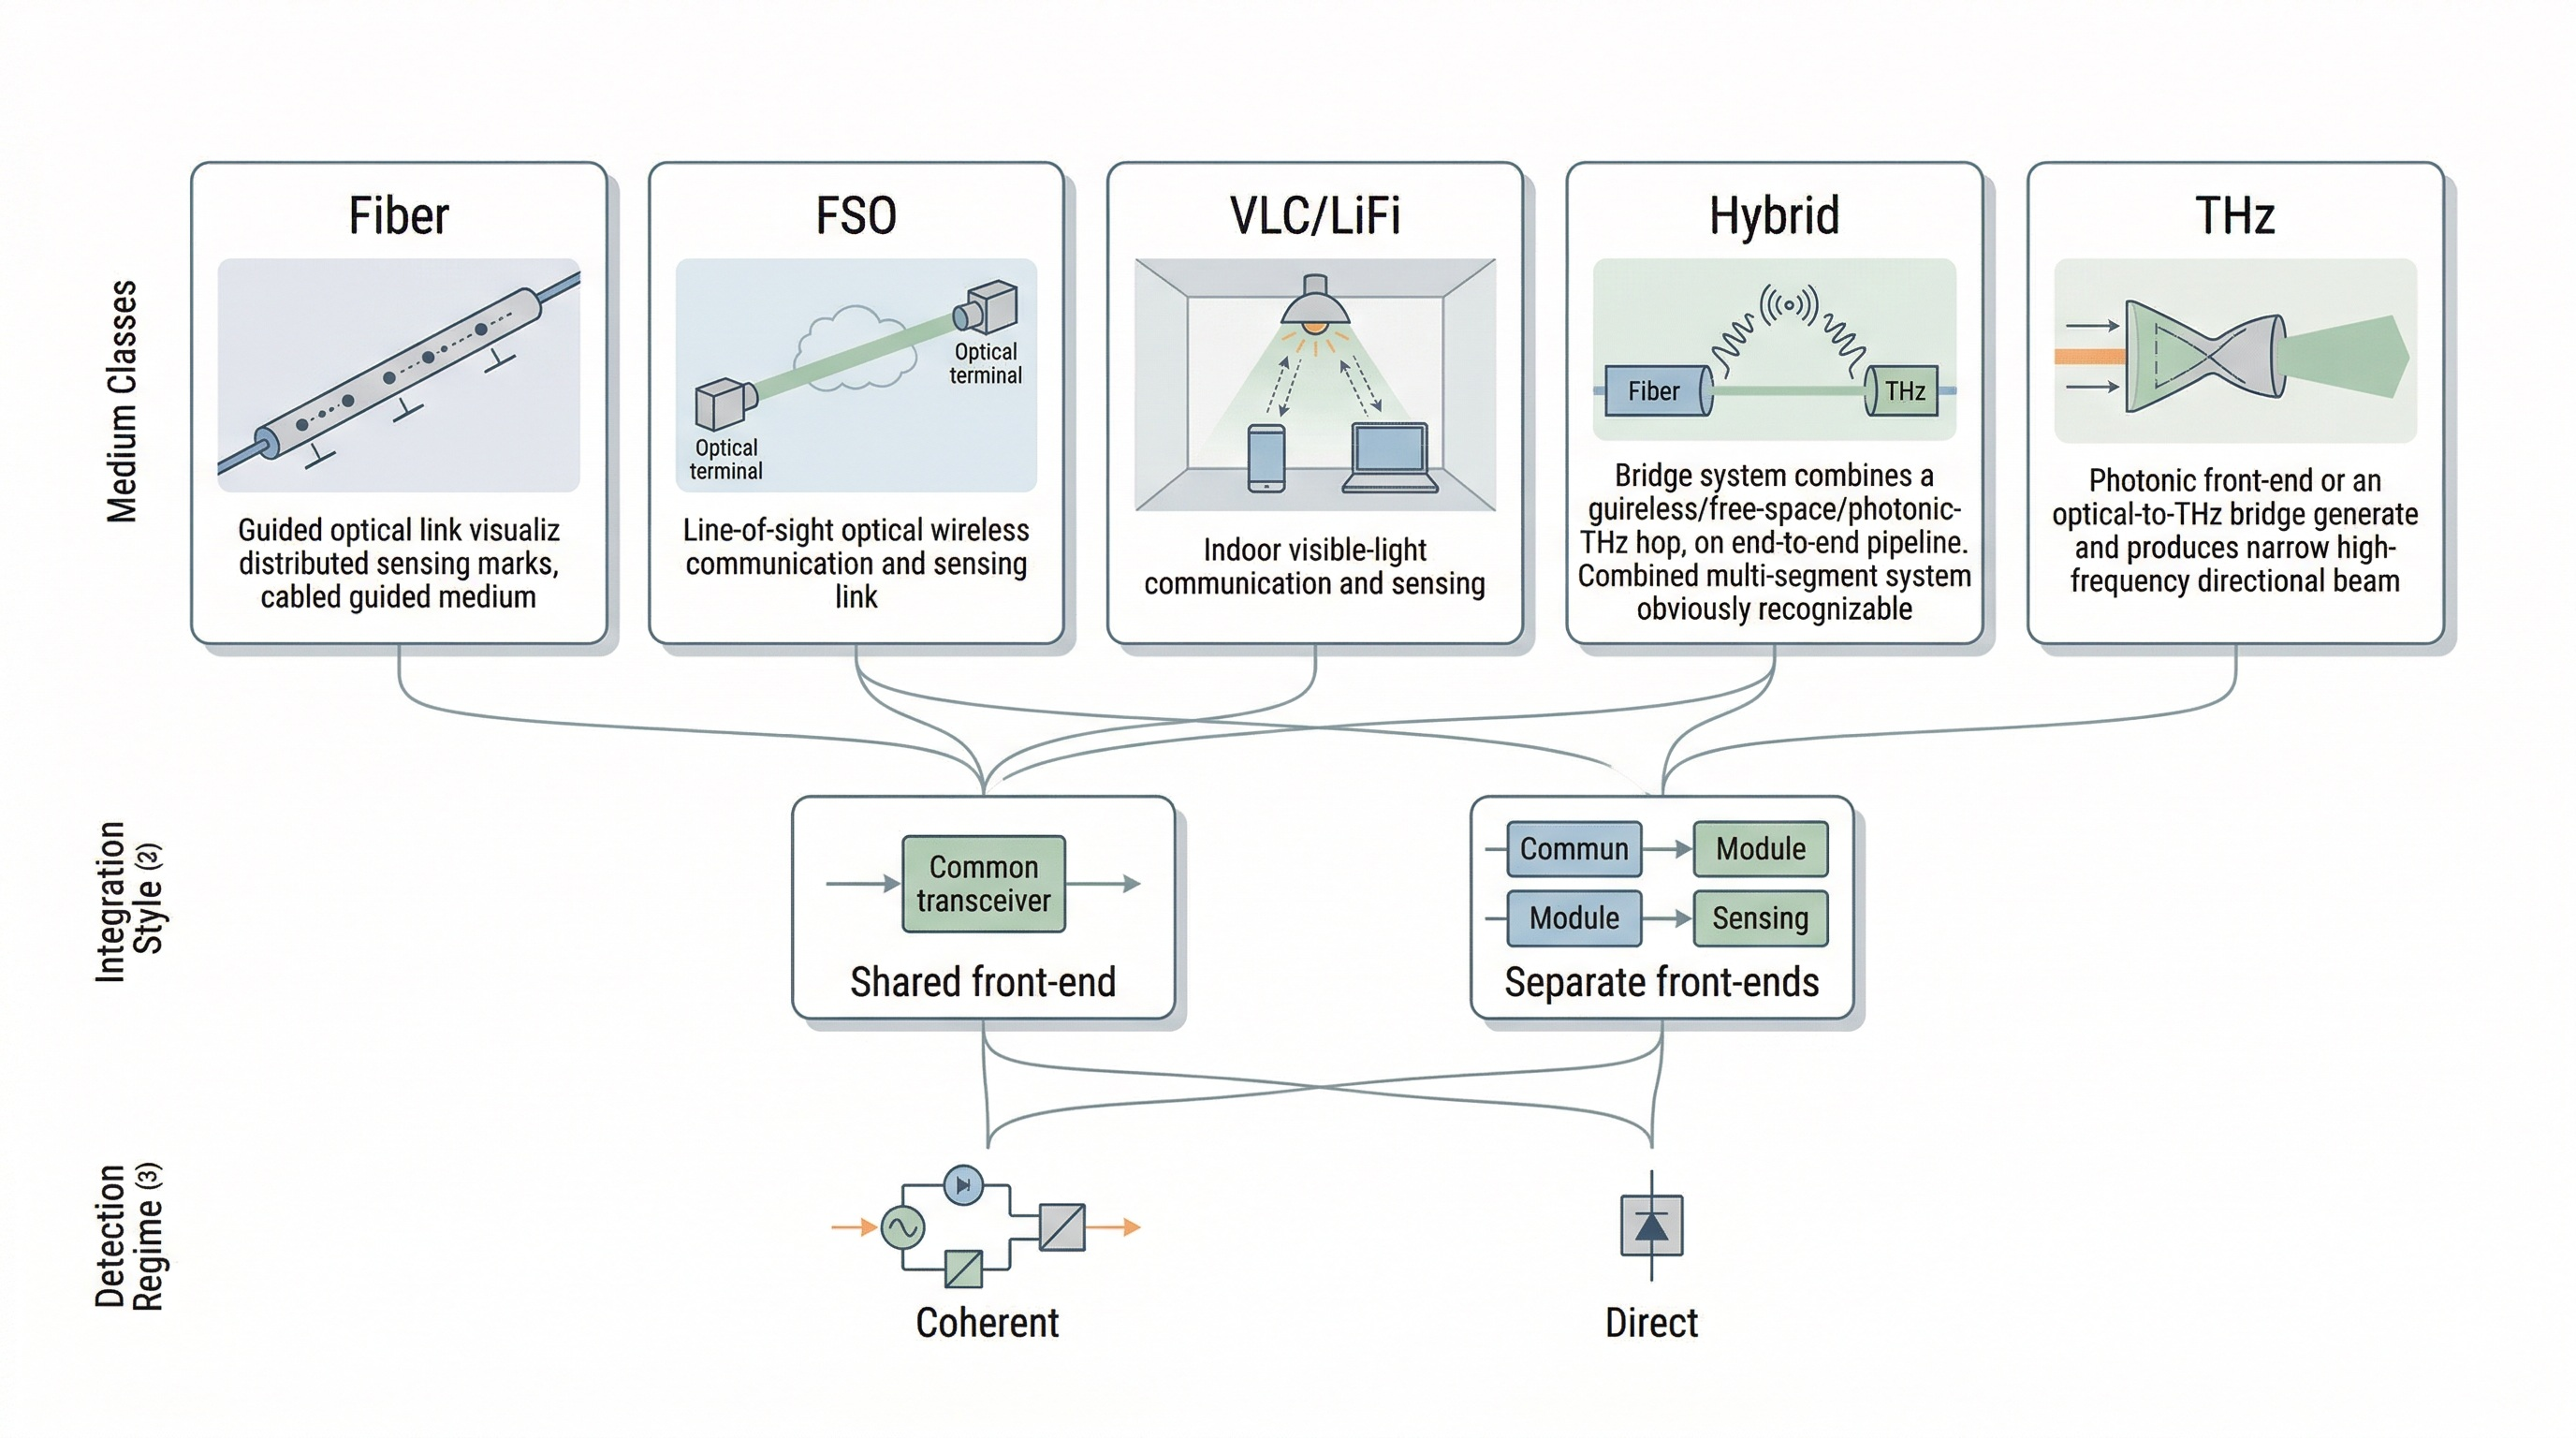
\includegraphics[width=\linewidth,trim=0.8cm 0.7cm 0.8cm 1.1cm,clip]{figures/fig_iv_1.jpg}
    \caption{Semantic taxonomy map retained as the single main-text taxonomy figure.}
    \label{fig:fig_iv_1}
\end{figure*}

\begin{table*}[!t]
    \caption{Compact taxonomy summary across the $N=220$ corpus.}
    \label{tab:taxonomy_compact}
    \centering
    \scriptsize
    \setlength{\tabcolsep}{2.7pt}
    \renewcommand{\arraystretch}{1.08}
    \begin{tabularx}{\textwidth}{@{}p{2.0cm}p{1.65cm}p{2.25cm}p{2.2cm}X@{}}
        \toprule
        Medium & Corpus share & Dominant detection & Dominant task & Governance warning \\
        \midrule
        Fiber & 45/220 & Coherent-leading, with direct tail & Range/vib. monitoring & Compare using guided-channel and $\Delta z$/OSNR semantics \\
        FSO & 19/220 & Mixed direct/coherent & Ranging-heavy & Condition on geometry, turbulence, and pointing assumptions \\
        VLC/LiFi & 25/220 & Direct IM/DD & Localization and ranging & Electrical-plane accuracy dominates; do not infer optical OSNR behavior \\
        Photonic-THz / hybrid & 116/220 hybrid; 39 photonic-THz anchors & Near-balanced coherent/direct & Ranging-heavy with broad multi-task tail & Separate optical generation/distribution from wireless propagation and receiver plane \\
        \bottomrule
    \end{tabularx}
\end{table*}

The medium axis is the first filter. Fiber O-ISAC is the guided anchor of the corpus, with 45 records. It includes distributed acoustic sensing, OFDR/DFOS-style monitoring, coherent communications with embedded sensing pilots, multicore or co-wavelength coexistence, and cabled infrastructure monitoring \cite{O_ISAC_006,O_ISAC_013,O_ISAC_020,O_ISAC_038,O_ISAC_041,O_ISAC_046,O_ISAC_069,O_ISAC_090}. The key interpretation rule is that fiber evidence is not a wireless ranging baseline. It is a guided-medium integration story in which OSNR, gauge length, spatial granularity, and interrogator assumptions often carry more meaning than free-space \(\Delta r_{\min}\).

FSO O-ISAC contains a smaller but important group of wireless optical records. It is strongly ranging-oriented and highly sensitive to link geometry, weather, turbulence, pointing, and blockage. FSO studies include DCO-OFDM, OCDM/FMCW-style waveform design, power allocation, remote phase-shift LiDAR with communication, retroreflective links, and UAV-aided or mixed FSO-RF designs \cite{O_ISAC_005,O_ISAC_023,O_ISAC_035,O_ISAC_040,O_ISAC_048,O_ISAC_051,O_ISAC_055,O_ISAC_099,O_ISAC_106}. Because FSO observability may be direct or coherent, its comparisons must remain receiver-model conditioned.

VLC/LiFi O-ISAC is the most direct-detection-heavy class. It includes indoor positioning, visible-light positioning and communication, LED-based joint systems, camera-assisted variants, gesture recognition, and multi-task learning under visible-light constraints \cite{O_ISAC_009,O_ISAC_022,O_ISAC_030,O_ISAC_039,O_ISAC_050,O_ISAC_054,O_ISAC_062,O_ISAC_068,O_ISAC_092,O_ISAC_110,O_ISAC_303,O_ISAC_327}. The evidence is often rich for localization and indoor services, but it is tied to illumination geometry, Lambertian channel assumptions, electrical SNR, and direct-detection noise. Those assumptions make VLC/LiFi valuable but not directly poolable with coherent fiber or photonic-THz records.

Photonic-THz and hybrid O-ISAC form the bridge class. The optical carrier may drive high-frequency generation, local oscillator distribution, fiber-wireless transport, coherent de-chirping, or THz-over-fiber operation, while the sensing target may lie in a high-frequency wireless channel \cite{O_ISAC_002,O_ISAC_016,O_ISAC_026,O_ISAC_029,O_ISAC_043,O_ISAC_044,O_ISAC_047,O_ISAC_057,O_ISAC_065,O_ISAC_070,O_ISAC_077,O_ISAC_105}. This class is especially tempting for rate--resolution headlines, so it requires strict plane separation: optical generation/distribution evidence, wireless propagation evidence, and post-detection signal-quality evidence are not the same object.

The integration axis distinguishes shared waveform, shared hardware, shared resources, and shared processing. Shared-waveform papers include OFDM/LFM/OCDM/OTFS-like structures where the same waveform carries communication and sensing information \cite{O_ISAC_035,O_ISAC_060,O_ISAC_075,O_ISAC_117,O_ISAC_188,O_ISAC_219,O_ISAC_259,O_ISAC_272}. Shared-hardware records expose common apertures, front-ends, photonic chips, or fiber links \cite{O_ISAC_036,O_ISAC_045,O_ISAC_061,O_ISAC_164,O_ISAC_324,O_ISAC_354,O_ISAC_360}. Shared-resource and shared-processing records express integration through time/frequency/power scheduling, beamforming, or inference pipelines \cite{O_ISAC_049,O_ISAC_052,O_ISAC_083,O_ISAC_086,O_ISAC_102,O_ISAC_134,O_ISAC_138,O_ISAC_140,O_ISAC_242,O_ISAC_340}.

The detection/observability axis prevents receiver-plane collapse. Direct IM/DD and coherent detection dominate the corpus, but the residual categories matter because they show that the field is not limited to a binary receiver taxonomy \cite{O_ISAC_001,O_ISAC_028,O_ISAC_029,O_ISAC_122,O_ISAC_136}. The sensing-task axis similarly separates ranging, localization, vibration/strain, environmental monitoring, object/gesture detection, and multi-task perception. Ambiguous records are retained with explicit tags rather than forced into a single dominant bucket. As a result, the taxonomy reports evidence concentration, not superiority.

\subsection{Taxonomy as a Guardrail, Not a Ranking}

The taxonomy is intentionally conservative. Its purpose is not to decide whether fiber, FSO, VLC/LiFi, or photonic-THz is the strongest O-ISAC platform. Each medium is solving a different version of the joint sensing-communication problem. Fiber has strong infrastructure relevance and mature optical transport machinery, but its sensing axis is often distributed and guided. FSO has clearer free-space ranging relevance but is highly scenario-sensitive. VLC/LiFi has a strong indoor localization and service-integration story but is dominated by direct-detection and illumination constraints. Photonic-THz/hybrid systems offer impressive rate and resolution demonstrations, yet they mix optical and wireless stages and therefore demand careful plane annotation.

The same logic applies to the integration axis. A shared waveform does not necessarily imply shared hardware, and a shared front-end does not necessarily imply a single optimization objective. Some papers integrate by embedding sensing pilots into communication signals. Others integrate by reusing optical carriers, apertures, front-end components, time-frequency resources, or DSP pipelines. The taxonomy keeps these mechanisms distinct because they create different tradeoffs. A shared waveform can create interference between sensing and communication symbols; shared hardware can create calibration and impairment coupling; shared resources can create scheduling tradeoffs; shared processing can create dataset and inference dependencies.

\subsection{Detection and Task Axes}

Detection/observability is the axis most closely tied to metric governance. Coherent systems may support phase-sensitive ranging, vibration, or de-chirping, while direct-detection systems may be more natural for intensity-domain localization, received-signal-strength inference, or simple ranging. A camera-assisted visible-light system may extract geometry in a different way again. For this reason, the taxonomy does not report direct and coherent systems as interchangeable variants of one receiver. They define different admissible comparisons.

The sensing-task axis further limits generalization. Ranging, localization, vibration, strain, environmental monitoring, gesture recognition, and target detection do not share one performance unit. A localization RMSE in an indoor VLC room is not a substitute for a fiber vibration spatial granularity, and neither is directly comparable with a photonic-THz range resolution unless the scenario and metric role are explicit. This is why later sections phrase application evidence as deployment motifs and Section~\ref{sec:tradeoff} separates rate--\(\Delta r_{\min}\), rate--\(\sigma_r\), and full-triplet subsets.

\subsection{How Ambiguity Is Retained}

Some records legitimately span multiple axes. A hybrid fiber-wireless paper may include optical generation, fiber distribution, wireless propagation, coherent reception, and DSP-based sensing. A VLC paper may combine direct photodiode reception with image-sensor or camera-assisted observability. A fiber study may report communication BER, OSNR, vibration recovery, and spatial granularity under one architecture. Rather than force such records into a single label, the extraction retains the dominant class and records ambiguity where it affects comparison. The result is a taxonomy that supports cautious synthesis and preserves the warning that prevalence is evidence concentration, not superiority.

\subsection{Additional Axis-Level Taxonomy Detail}

The four-axis taxonomy is used as a comparability guardrail rather than a ranking mechanism. At corpus level, the dominant medium labels are hybrid 116/220, fiber 45/220, VLC/LiFi 25/220, FSO 19/220, and terahertz 1/220, with the remaining records forming a heterogeneous long tail. Shared front-end integration appears in 194/220 records, detection labels are concentrated in direct 118/220 and coherent 97/220 records, and ranging is the most common task label at 162/220. These counts indicate evidence concentration, not superiority: any cross-paper comparison still requires the Section~\ref{sec:background_metric_contract} distinctions among medium, receiver observability, metric role, and signal-quality plane.

The medium axis is therefore not a maturity ranking. The hybrid majority reflects how often optical generation, fiber distribution, wireless propagation, or mixed front-end chains appear together in the literature. It does not mean that hybrid platforms are universally more mature than fiber, FSO, or VLC/LiFi. Fiber records are fewer but often more concrete for guided infrastructure monitoring and transport coexistence. VLC/LiFi records are fewer again but define a distinct direct-detection indoor service class. FSO records remain scenario-sensitive because geometry, turbulence, pointing, and visibility conditions dominate interpretation. The taxonomy keeps these classes separate so that later sections can discuss transfer without erasing the deployment assumptions that make each class meaningful.

The integration axis serves a different purpose. A shared front end is common, but it does not by itself prove that communication and sensing are optimized together. Some records share apertures, fiber paths, photonic components, or receiver chains while keeping communication and sensing tasks analytically separate. Others share waveform, resource, or processing layers more directly. For this reason, the taxonomy treats integration mechanism as an evidence descriptor rather than a binary label. The important question is not simply whether a system is "integrated", but which physical or algorithmic layer carries the integration burden and which metrics reveal the resulting tradeoff.

The detection and task axes are the bridge to metric governance. A direct-detection VLC/LiFi localization study and a coherent photonic-THz ranging study may both report optical O-ISAC results, but they expose different observables and different error mechanisms. Likewise, a ranging task, a localization task, a vibration-monitoring task, and an environmental-sensing task do not share one natural endpoint. The taxonomy therefore provides the conditioning variables that Section~\ref{sec:tradeoff} later needs. It tells the reader which comparisons are plausible, which require explicit receiver-plane conversion, and which should remain modality-specific evidence.

\section{Communication-Sensing Tradeoff Synthesis}
\label{sec:tradeoff}

The governed tradeoff synthesis is the core analytical contribution. The extraction produced 225 scenario points from the \(N=220\) paper corpus. Raw metric coverage initially appears broad because many papers report at least one communication metric and at least one sensing metric. Under the governance contract, however, a point is usable only when the relevant metrics belong to a compatible scenario record and the metric role is clear. After filtering, only 20 scenario records support rate plus \(\Delta r_{\min}\), only 16 support rate plus \(\sigma_r\)/RMSE, and only 13 support the full rate--\(\Delta r_{\min}\)--\(\sigma_r\) triplet. This attrition is the central result.

\begin{table*}[!t]
    \caption{Governance attrition from reported metrics to admissible synthesis.}
    \label{tab:governance_attrition}
    \centering
    \scriptsize
    \setlength{\tabcolsep}{3pt}
    \renewcommand{\arraystretch}{1.08}
    \begin{tabularx}{\textwidth}{@{}p{2.8cm}p{2.0cm}p{2.2cm}X@{}}
        \toprule
        Evidence layer & Available count & Main retained use & Main attrition cause \\
        \midrule
        Scenario records & 225 & Corpus-level context & Heterogeneous reporting and modality planes \\
        Rate + $\Delta r_{\min}$ & 20 & CRQ-admissible resolution view & Missing matched bandwidth-limited resolution \\
        Rate + $\sigma_r$/RMSE & 16 & Accuracy-conditioned operating view & Missing estimator/SNR/geometry detail \\
        Full triplet & 13 & Most conservative cross-metric subset & Rate, resolution, and accuracy rarely co-reported \\
        \bottomrule
    \end{tabularx}
\end{table*}

\begin{figure*}[!t]
    \centering
    
\includegraphics[width=\linewidth]{figures/fig_v_1.png}
    \caption{Governed rate--resolution and rate--accuracy operating clouds after metric-role filtering.}
    \label{fig:fig_v_1}
\end{figure*}

The first governed view uses rate and \(\Delta r_{\min}\). This view is admissible for records that disclose a bandwidth-limited resolution quantity tied to the same scenario as the reported rate. Photonic-THz and fiber-wireless demonstrations are prominent in this view because they often report high rates and fine delay/ranging resolution in one experiment \cite{O_ISAC_016,O_ISAC_026,O_ISAC_029,O_ISAC_043,O_ISAC_044,O_ISAC_065,O_ISAC_070,O_ISAC_077,O_ISAC_105}. Yet even here, the evidence is sparse compared with the full corpus, and the view should not be interpreted as a universal frontier.

The second governed view uses rate and \(\sigma_r\)/RMSE. This view is different because it is estimator-level and often geometry- or SNR-dependent. VLC/LiFi localization and FSO resource-allocation studies can be important here, but only when the estimation metric, scenario, and signal-quality plane are clear \cite{O_ISAC_009,O_ISAC_023,O_ISAC_039,O_ISAC_050,O_ISAC_052,O_ISAC_054,O_ISAC_061,O_ISAC_062}. A small \(\sigma_r\) value is not automatically comparable with a small \(\Delta r_{\min}\), and a CRB/FIM bound is not a measured RMSE. Fig.~\ref{fig:fig_v_1} therefore separates the operating clouds rather than overlaying all sensing values.

\begin{table*}[!t]
    \caption{Governed fiber, wireless, and hybrid slices.}
    \label{tab:comparative_slices}
    \centering
    \scriptsize
    \setlength{\tabcolsep}{2.8pt}
    \renewcommand{\arraystretch}{1.08}
    \begin{tabularx}{\textwidth}{@{}p{1.7cm}p{2.0cm}p{2.1cm}X@{}}
        \toprule
        Slice & Strong evidence & Weakness for pooling & Main reading \\
        \midrule
        Fiber & Tb/s-class aggregate links and distributed sensing \cite{O_ISAC_046} & $\Delta z$ and OSNR differ from wireless range/ESNR & Guided infrastructure and monitoring anchor \\
        Wireless optical & FSO/VLC ranging/localization and OPA-controlled optical wireless links \cite{O_ISAC_023,O_ISAC_061} & Geometry, turbulence, ambient light, and estimator differences & Scenario-conditioned sensing/communication tradeoff \\
        Photonic-THz/hybrid & High-rate photonic generation plus mmWave/THz ranging \cite{O_ISAC_029,O_ISAC_105} & Optical and wireless planes can be conflated & Bridge class, not a single medium \\
        \bottomrule
    \end{tabularx}
\end{table*}

Table~\ref{tab:comparative_slices} highlights why naive pooling is unsafe. Fiber records can dominate communication capacity or infrastructure monitoring relevance, but their sensing granularity and OSNR semantics differ from wireless range/accuracy metrics \cite{O_ISAC_038,O_ISAC_041,O_ISAC_046,O_ISAC_069,O_ISAC_074}. Wireless optical records often expose clearer ranging/localization tasks but are more sensitive to geometry, channel, and receiver assumptions \cite{O_ISAC_003,O_ISAC_005,O_ISAC_023,O_ISAC_035,O_ISAC_039,O_ISAC_048}. Photonic-THz/hybrid records provide many high-rate, high-frequency anchors, but they mix optical and wireless stages and must be read through the measurement-plane contract \cite{O_ISAC_026,O_ISAC_029,O_ISAC_047,O_ISAC_065,O_ISAC_077,O_ISAC_105}.

The CRQ-valid subset is therefore sparse and illustrative. CRQ is informative when \(R\) and \(\Delta r_{\min}\) are matched, but it is not a stable design envelope for the field. The current evidence says more about reporting practice than about ultimate physical limits: many O-ISAC studies do not report the rate, bandwidth-limited resolution, estimator-level accuracy, receiver plane, and scenario fields needed for full cross-metric synthesis. A future benchmark culture should close this reporting gap before broad optical-ISAC frontiers are claimed.

\subsection{Why Raw Coverage Overstates Comparability}

If one counts only whether papers mention communication and sensing, the O-ISAC evidence base appears much denser than it is. Many records report a rate, BER, SE, throughput, OSNR, received power, or modulation result, and many also report a sensing quantity. The difficulty is that these quantities are often not attached to the same scenario, not expressed in the same metric role, or not accompanied by enough receiver-plane detail. A paper may report a communication rate in one operating mode and a sensing resolution in another; another may provide a CRB curve without measured accuracy; a third may report fiber spatial granularity and communication OSNR but no wireless range-resolution equivalent. These are useful results, but they cannot all enter a single frontier.

The governed attrition in Table~\ref{tab:governance_attrition} should therefore be read as a reproducibility signal. The field is not short of promising demonstrations. It is short of reporting patterns that allow the demonstrations to be compared without hidden substitutions. The 20 rate--\(\Delta r_{\min}\) points are the subset in which a rate and a bandwidth-limited resolution are co-reported with sufficient scenario alignment. The 16 rate--\(\sigma_r\)/RMSE points are the subset in which rate and estimator-level accuracy are co-reported. The 13 full-triplet records are the most conservative subset because they support both physical-resolution and estimator-accuracy readings.

\subsection{Resolution, Accuracy, and Bound-Level Evidence}

The separation between \(\Delta r_{\min}\), \(\sigma_r\)/RMSE, and CRB/FIM is not semantic hair-splitting. \(\Delta r_{\min}\) answers a physical bandwidth question: given an effective bandwidth and propagation convention, what is the nominal resolvable range separation? \(\sigma_r\) or RMSE answers an estimator performance question: under a particular SNR, geometry, dataset, or algorithm, how far is the estimate from the truth? CRB/FIM answers a bound question: under a model and noise assumption, what lower bound applies to an unbiased estimator? These answers can be related inside one paper, but they are not exchangeable across papers unless the model and scenario are aligned.

This is why the review does not report a single sensing column for all O-ISAC records. A photonic-THz system with very fine \(\Delta r_{\min}\) can be a strong bandwidth-limited ranging example, but its value does not make a VLC localization RMSE irrelevant. A fiber system with excellent spatial monitoring can be central to infrastructure O-ISAC, but its \(\Delta z\) cannot become a wireless range-resolution point. A CRB/FIM study can clarify theoretical limits, but it cannot replace measured or simulated RMSE in the governed rate--accuracy cloud. The Section~\ref{sec:tradeoff} synthesis is therefore deliberately plural.

\subsection{Fiber, Wireless Optical, and Hybrid Slices}

The fiber slice is strongest when interpreted as guided infrastructure sensing integrated with optical communication. It includes high-capacity transport, distributed vibration or strain monitoring, and coexistence mechanisms that share wavelength, fiber, or DSP resources. Its communication evidence can be extremely strong, but its sensing evidence is often spatially distributed rather than target-ranging. This makes fiber essential to O-ISAC while also making naive pooling unsafe.

The wireless optical slice includes FSO and VLC/LiFi systems. FSO is often closer to a free-space ranging formulation and may report bandwidth-limited resolution, Fisher information, or power-allocation tradeoffs. VLC/LiFi is frequently localization- or indoor-service-oriented, and its direct-detection receiver makes electrical-plane SNR and room geometry central. These two wireless optical subclasses should not be merged blindly: FSO and VLC both propagate optically through air, but their deployment constraints and receiver models differ.

The photonic-THz/hybrid slice is the most important bridge for high-rate rate--resolution claims. It often combines optical generation, fiber distribution, high-frequency wireless propagation, and coherent or electronic reception. This architecture can produce impressive CRQ values, but the bridge nature also creates a governance hazard. The communication rate may be measured through a fiber-wireless link, the sensing resolution may be tied to a high-frequency waveform, and the signal-quality plane may move from optical to electrical to DSP stages. For that reason, the review treats this class as a bridge rather than a homogeneous medium bucket.

\subsection{Interpretation of the Sparse CRQ Subset}

The sparse CRQ-valid subset should be interpreted in two ways. Technically, it shows that a small number of O-ISAC demonstrations jointly report high rate and bandwidth-limited resolution under matched scenarios. Methodologically, it shows that most of the corpus cannot yet support CRQ comparison because the required fields are absent or unmatched. The second point is the stronger COMST contribution. A field can have many strong demonstrations and still lack the reporting discipline needed for cross-paper synthesis.

This also prevents overclaiming a Pareto frontier. The point clouds and CRQ subset are fixed-case summaries of reported scenarios. They are not optimized over hardware cost, power, aperture, waveform, environment, receiver complexity, or deployment domain. A nondominated point in the sparse subset is not a universal design envelope; it is an informative reported scenario under the review's admissibility rules. Future O-ISAC benchmarks should make this distinction explicit by reporting matched rate, \(\Delta r_{\min}\), \(\sigma_r\)/RMSE, CRB/FIM context, \(\Delta z\) when relevant, and signal-quality plane in the same record.

\subsection{Additional Tradeoff Interpretation}

Section V-A works on governed scenario records rather than raw study counts. Communication metrics are scoped to reported communication rate ($R$) and link-quality indicators, with strict separation between optical-plane OSNR and electrical-plane SNR/ESNR because the two are measured at different receiver-chain stages. Table~\ref{tab:governance_attrition} summarizes the resulting plane-aware coverage.

Before governance filtering, communication reporting appears broad: the 225-point trade-off set includes rate in 197 records, electrical-plane SNR in 190, and optical-plane OSNR in 169. After the Section II filter, however, only 53/225 scenarios remain usable, 172 are blocked, and 169 papers lose all scenarios. The dominant blocker is metric-plane mixing (169 records), followed by $\Delta z$-to-$\Delta r_{\min}$ aliasing (19 records, with 16 overlapping both flags). Within the governed subset, rate-bearing records are concentrated in hybrid (17) and cabled fiber (12), yielding medians of 10 Gbps and 28.5 Gbps, respectively; the remaining media are sparse and should be read as anchors rather than distributions. Electrical-plane SNR survives in only 20 governed records, while governance-usable OSNR drops to zero, so Section V-A can support electrical-plane quality remarks but not optical-plane cross-medium comparisons. CRQ-linked comments are likewise bounded to the 20 eligible records, dominated by hybrid (14) and cabled fiber (4). The same pattern explains the section's conservatism overall: the governance audit reports 299 MAJOR violations across 169 papers, including 261 metric-plane and 38 metric-aliasing violations, so communication synthesis remains intentionally selective rather than coverage-maximizing.

Section V-B keeps the same governed scenario scope but reorganizes sensing evidence by function rather than by lexical surface form. $\Delta r_{\min}$ represents physical resolution, $\sigma_r$ estimator-level accuracy, CRB bound-level context, and $\Delta z$ fiber spatial granularity; these roles are not interchangeable, so Table~\ref{tab:governance_attrition} reports them separately and Fig.~\ref{fig:fig_v_1} preserves distinct resolution and accuracy layers.

Before governance filtering, sensing coverage is broad: across 225 scenario points, $\Delta r_{\min}$ appears in 195 records, $\Delta r_{\min}$-eligible reporting in 173, $\sigma_r$ in 186, CRB in 148, and $\Delta z$ in 161, with similarly high paper-level coverage. After filtering, however, only 53/225 scenarios remain usable overall. At role level, only 20/173 $\Delta r_{\min}$-eligible records and 16/186 $\sigma_r$ records survive, while both CRB and $\Delta z$ fall to zero usable entries. The exclusion pattern is highly structured rather than random: 151/153 blocked $\Delta r_{\min}$-eligible records, 169/170 blocked $\sigma_r$ records, and 147/148 blocked CRB records are plane-mixed. The synthesis therefore separates reported coverage from governance-usable coverage because raw prevalence overstates comparative readiness.

Within the governed subset, $\Delta r_{\min}$-eligible points are concentrated in hybrid (14) and cabled fiber (4), with single anchors in wireless FSO and terahertz; across all usable points, $\Delta r_{\min}$ spans 0.0025--15 m with a median of 0.0397 m. Estimator-level accuracy is even sparser: only 16 usable records report $\sigma_r$ (hybrid 8, cabled fiber 7, terahertz 1), spanning 0.001--1000 m with a median of 0.0575 m, and only 13 usable records contain both $\Delta r_{\min}$ and $\sigma_r$. This asymmetry is why Fig.~\ref{fig:fig_v_1} keeps separate resolution and accuracy panels. CRB and $\Delta z$ remain contextual only, because neither survives governance filtering; OSNR is likewise absent from the usable sensing subset, whereas electrical-plane SNR remains available in 12/20 $\Delta r_{\min}$-eligible and 14/16 $\sigma_r$ records. The same conservatism also matches the qualitative trade-off record: DIRECT articulation exists, but it remains a minority pattern relative to total mention volume, and the 299 MAJOR governance violations across 169 papers continue to limit synthesis-ready support.

Section V-C is the synthesis core of the section: it converts the governed metric subsets into operating-cloud and frontier-style views without relaxing the Section II contract. Rate-versus-resolution is interpreted through rate and $\Delta r_{\min}$, rate-versus-accuracy through rate and $\sigma_r$, while CRB remains bound-level context and $\Delta z$ is never used as a surrogate for $\Delta r_{\min}$. The main figure therefore keeps the resolution and accuracy layers separate, while the CRQ discussion is bounded to the valid subset.

The full trade-off table contains 225 scenario points from 220 papers, but the governed subset is much smaller: only 20 points support rate-plus-$\Delta r_{\min}$ interpretation and 16 support rate-plus-$\sigma_r$, with only 13 supporting the full triplet. This contraction is not cosmetic; it determines the admissible evidence for trade-off inference. Labels remain useful narrative cues, but dimensional interpretation is grounded in governed metric availability rather than label strings alone. The governed operating region is still numerically informative: rate spans 25 Mbps to 448 Gbps (median 10 Gbps), $\Delta r_{\min}$ spans 0.0025--15 m (median 0.0397 m), and $\sigma_r$ spans 0.001--1000 m (median 0.0575 m). Coupling-mode coverage is likewise asymmetric, with \texttt{resource\_division} dominant in both the raw and governed sets.

CRQ filtering makes the admissibility compression even clearer. The point taxonomy is 225 total points, 170 CRQ-candidate points, 20 CRQ-valid points, and only 2 Pareto points. The 20 valid points are distributed across hybrid (14), cabled fiber (4), terahertz (1), and wireless FSO (1), with CRQ spanning $6.67 \times 10^8$ to $4.8 \times 10^{13}$ bps/m and a median of $4.33 \times 10^{10}$ bps/m. Because the frontier itself contains only one hybrid and one wireless FSO point, this view should be read as a bounded illustrative frontier rather than a stable design envelope. The same caveat applies to measurement-plane conditioning: electrical-plane SNR remains available in part of the governed subset, but governance-usable OSNR remains absent throughout.

Trade-off-language extraction is consistent with this conservatism: explicit trade-off reasoning exists, but DIRECT articulation remains a minority pattern relative to total mention volume. The same 299 MAJOR governance violations across 169 papers therefore remain central to interpretation in V-C, because they explain much of the candidate-to-valid compression and the sparsity of the Pareto set.

Section V-D keeps the same governed scenario scope but changes the question from ``what is available?'' to ``what can be compared responsibly?''. Medium labels remain exactly as normalized in Section IV, hybrid is retained as a bridge class rather than forced into either endpoint, and Table~\ref{tab:comparative_slices} is the primary comparative anchor.

The contraction from raw to governed evidence directly shapes what can be compared. The raw trade-off set contains 225 scenario points across 12 medium labels, but governance filtering retains only 53, distributed mainly across hybrid (27), cabled fiber (15), and smaller wireless slices. Within that governed set, fiber contributes 15 points from 13 papers, wireless 9 points from 9 papers, and hybrid 27 points from 27 papers. Metric completeness is asymmetric: fiber contributes 12 rate values, 4 $\Delta r_{\min}$ values, and 7 $\sigma_r$ values; wireless contributes 3, 1, and 0; hybrid contributes 17, 14, and 8. The comparative slice should therefore be read as a constrained synthesis over a reduced admissible set rather than as a mirror of raw-corpus prevalence.

The governed medians suggest different operating emphases, but not universal superiority claims. Fiber shows a median rate of 28.5 Gbps, wireless 1 Gbps, and hybrid 10 Gbps, yet the wireless slice is structurally unstable because it is sparse and heterogeneous. Sensing-side comparison is even more asymmetric: fiber has median $\Delta r_{\min}=5.5$ m and median $\sigma_r=0.1$ m, wireless has only one governed $\Delta r_{\min}$ value and no governed $\sigma_r$, and hybrid supports both metrics with medians of 0.019075 m and 0.01 m. CRQ comparison is similarly bounded to the 20 eligible points, while electrical-plane SNR remains available only for fiber, hybrid, and one wireless anchor. V-D is therefore intentionally conservative: it preserves comparison where support exists, keeps hybrid explicit, and treats sparse slices as non-ranking evidence.

\subsection{Benchmark Implications of Governed Attrition}

The governed attrition result should be read as a design requirement for future O-ISAC reporting. The corpus does not merely need more headline rates or more sensing demonstrations; it needs records in which the communication and sensing quantities are tied to the same operating point. A benchmark-quality record should state the medium, integration mechanism, receiver observability, geometry, waveform or bandwidth convention, signal-quality plane, communication endpoint, and sensing endpoint before presenting a rate--sensing tradeoff. Without those fields, the result may still be valuable as a modality-specific demonstration, but it cannot enter the cross-paper synthesis used here.

The first practical implication is scenario coupling. Rate, resolution, and accuracy values should be reported for the same link, waveform, aperture, receiver, and environmental condition. If a paper reports a high data rate under one modulation or beam state and a fine sensing value under another, both values remain useful, but they do not define a governed rate--resolution point. The Section~\ref{sec:tradeoff} ledger therefore treats unmatched values as separate evidence rather than combining them into a synthetic frontier. This rule is conservative by design: it prevents a survey from creating an apparent tradeoff curve that no individual experiment or simulation actually reported.

The second implication is metric-role disclosure. A bandwidth-limited $\Delta r_{\min}$ value should be accompanied by the effective bandwidth and propagation convention that define it. An estimator-level $\sigma_r$ or RMSE value should be accompanied by the estimator, SNR or OSNR/SNR plane, geometry, dataset or simulation setup, and uncertainty convention. A CRB/FIM value should state the observation model and parameterization because it is a bound-type object rather than measured error. A fiber $\Delta z$ value should disclose gauge length, segment spacing, or interrogator assumptions because it is a guided spatial granularity rather than wireless range resolution. These disclosures are not cosmetic; they determine which columns of Table~\ref{tab:governance_attrition} a record can enter.

The third implication is measurement-plane discipline. Optical systems often move through several physical and signal-processing stages: optical generation, guided distribution, wireless propagation, photodetection, electrical amplification, digitization, and DSP. A single value labeled SNR can refer to different locations in that chain, and an OSNR value before coherent reception is not interchangeable with electrical SNR after direct detection. The governed synthesis therefore rejects plane-mixed records even when their numerical values look compatible. This is why OSNR can be widespread in the raw corpus yet unavailable for the governed cross-medium sensing subset.

The fourth implication concerns medium-specific transfer. Fiber, FSO, VLC/LiFi, and photonic-THz/hybrid studies can inform one another, but only after their measurement roles are exposed. Fiber work contributes strongly to guided infrastructure monitoring and optical transport coexistence; FSO work contributes geometry- and atmosphere-conditioned free-space optical ranging; VLC/LiFi work contributes direct-detection indoor localization and service integration; photonic-THz/hybrid work contributes high-frequency waveform generation and fiber-wireless bridge architectures. These are complementary bodies of evidence, not interchangeable samples from one distribution. A future benchmark suite should therefore define several scenario families rather than one universal optical-ISAC channel.

The fifth implication is that negative space should be reported explicitly. A paper may not report $\sigma_r$, may not disclose a bandwidth convention for $\Delta r_{\min}$, or may not provide enough receiver-plane information to convert an SNR value. In current practice, such omissions often disappear inside prose summaries. For a systematic survey, however, the absence is itself informative: it explains why a study supports taxonomy, enabler, or application synthesis but not CRQ synthesis. A benchmark culture should make this status visible by including "not reported" and "not comparable" fields rather than forcing every paper into every metric column.

This reading also clarifies why the sparse CRQ-valid subset is not a negative judgment on O-ISAC technology. Several optical platforms demonstrate strong communication and sensing potential. The finding is instead that only a small subset reports the matched fields required for cross-paper numerical governance. The field can improve this quickly without waiting for a single dominant architecture: authors can report matched scenarios, annotate receiver planes, separate physical resolution from estimator accuracy, and publish extraction-friendly parameter tables. These practices would enlarge the governed subset and make future COMST-style updates more quantitative without weakening the modality distinctions protected in this review.

Finally, the governed synthesis should guide how claims are worded. A record can be described as a high-rate photonic-THz ranging demonstration, a guided-fiber monitoring and transport coexistence demonstration, or an indoor VLC/LiFi localization demonstration without being forced into a universal O-ISAC ranking. When the matched fields are present, the record can also support rate--$\Delta r_{\min}$, rate--$\sigma_r$, or full-triplet comparison. When they are absent, the record still belongs in the systematic review but should be assigned to a narrower evidence role. This evidence-role separation is the main reason Section~\ref{sec:tradeoff} is kept as the protected core of the manuscript.

\subsection{Reading Rules for the Section V Evidence}

The Section V evidence is most useful when read as a set of admissibility layers. The first layer is corpus membership: a paper can belong to the O-ISAC review because it integrates, coexists, or jointly discusses optical communication and sensing. The second layer is taxonomy support: the same paper can help establish the medium, integration, detection, and sensing-task distribution even if it reports no matched numerical tradeoff. The third layer is metric support: a paper can report a rate, a sensing value, or a signal-quality value that is meaningful within its own modality. The fourth layer is governed synthesis support: only records that attach compatible metrics to the same scenario enter the rate--sensing comparison. Confusing these layers is the fastest way to overstate the maturity of the field.

This layered reading explains why the full \(N=220\) corpus and the smaller governed subset should not be treated as competing facts. The large corpus establishes systematic coverage and shows that O-ISAC is active across fiber, FSO, VLC/LiFi, photonic-THz, and hybrid platforms. The smaller governed subset identifies how much of that activity is currently ready for direct numerical synthesis. Both statements are needed. A short corpus would not justify a cross-modality survey; a large corpus without governed filtering would encourage unsafe comparison. The contribution of this review is to keep the two levels visible at the same time.

The same logic applies to the 225 scenario points. They are not 225 interchangeable operating points, because several papers contain more than one scenario and because scenarios differ in medium, receiver, geometry, waveform, and metric plane. The point count is therefore a structured extraction count, not a pooled experimental sample. Governance filtering asks whether each point has the fields needed for a particular comparison. This is why one point can support rate-only interpretation, another can support sensing-only interpretation, and only a small subset can support rate--resolution or rate--accuracy synthesis.

The governed rate--$\Delta r_{\min}$ subset should be read as a physical-resolution subset. It is appropriate when the sensing quantity is tied to bandwidth and propagation convention, and when the rate is reported for the same scenario. It is not appropriate when a paper reports only localization RMSE, a CRB curve, fiber spatial granularity, or a sensing value from a different operating mode. Similarly, the governed rate--$\sigma_r$/RMSE subset should be read as an estimator-performance subset. It is appropriate when the accuracy metric is tied to the same scenario and the receiver/noise conditions are sufficiently clear. It is not a substitute for $\Delta r_{\min}$.

The full-triplet subset is the most restrictive because it asks for both physical-resolution and estimator-accuracy readings alongside rate. This requirement is demanding but important. A system can have a fine theoretical range resolution and still have poor estimator accuracy under low SNR, poor geometry, or model mismatch. Conversely, a system can report good empirical accuracy without disclosing a bandwidth-limited resolution convention. When all three quantities are present under one scenario, the reader can begin to separate physical bandwidth, estimator behavior, and communication performance. The fact that only 13 records support this full reading is therefore a reporting result, not a technology ranking.

For authors of future O-ISAC studies, the practical checklist is short. Report the optical medium and any hybrid wireless stage. State whether the receiver is coherent, IM/DD, camera-assisted, or otherwise observable. Give the communication rate, bandwidth, BER or throughput convention, and signal-quality plane. For sensing, state whether the main value is $\Delta r_{\min}$, $\sigma_r$/RMSE, CRB/FIM, $\Delta z$, or another task-specific endpoint. Keep all of these values tied to the same scenario table. If multiple scenarios are studied, report them as separate rows rather than mixing best-case values. This would turn many currently useful but non-governed records into synthesis-ready evidence.

For readers, the checklist is equally important. A high CRQ value should prompt the question of whether \(R\) and \(\Delta r_{\min}\) are matched and whether the scenario is comparable to the intended deployment. A small RMSE should prompt the question of geometry, estimator, SNR plane, and dataset or simulation conditions. A CRB should prompt the question of model assumptions. A fiber spatial granularity should prompt the question of gauge length and interrogator configuration rather than free-space range. These questions are the review's defense against converting heterogeneous O-ISAC demonstrations into a misleading single leaderboard.

\section{Enabling Technologies and System-Level Co-Design}
\label{sec:enablers}

O-ISAC enablers matter because they determine whether the metric-governed taxonomy can become deployable systems. The main enabler families are ORIS/optical RIS, OPA, PIC and photonic integration, photonics-assisted mmWave/THz generation, and ML/security-aware adaptation. Table~\ref{tab:vi_a_enablers} keeps the synthesis compact while the surrounding prose explains what each family contributes and what must be reported.

\begin{table*}[!t]
    \caption{Compact enabler synthesis for O-ISAC.}
    \label{tab:vi_a_enablers}
    \centering
    \scriptsize
    \setlength{\tabcolsep}{2.8pt}
    \renewcommand{\arraystretch}{1.08}
    \begin{tabularx}{\textwidth}{@{}p{2.15cm}p{2.65cm}p{2.3cm}X@{}}
        \toprule
        Enabler & Main O-ISAC role & Evidence center & Reporting risk \\
        \midrule
        ORIS / optical RIS & Programmable reflection, beam control, spatial reuse & Optical wireless and RIS-adjacent ISAC \cite{O_ISAC_163} & Geometry and control overhead must be disclosed \\
        OPA & Beam steering and joint communication/sensing aperture & OPA-based optical wireless ISAC \cite{O_ISAC_061,O_ISAC_091} & Beam pattern, scan schedule, and sensing estimator must be linked \\
        PIC / photonic integration & Compact source/modulator/receiver integration & Fiber-wireless and chip-scale demonstrations \cite{O_ISAC_036,O_ISAC_045} & Device results need system-level metric planes \\
        Photonics-assisted mmWave/THz & High-frequency generation/distribution and coherent reception & W-band, D-band, and THz-over-fiber systems \cite{O_ISAC_029,O_ISAC_070} & Separate optical generation from wireless propagation \\
        ML/security adaptation & Inference, calibration, robustness, and attack-aware control & Learning-assisted VLC/fiber-wireless studies \cite{O_ISAC_039,O_ISAC_242} & Dataset, generalization, and threat model must be explicit \\
        \bottomrule
    \end{tabularx}
\end{table*}

ORIS and optical RIS concepts promise programmable optical reflection, beam shaping, and spatial reuse. They are most naturally connected to optical wireless deployments where geometry, blockage, or coverage can be controlled by reconfigurable surfaces \cite{O_ISAC_112,O_ISAC_145,O_ISAC_156,O_ISAC_163,O_ISAC_200}. Their O-ISAC value depends on reporting the surface model, phase/amplitude control assumptions, alignment burden, and whether sensing observes the same controlled path as communication.

OPA technologies provide aperture-level beam steering for optical wireless ISAC. OPA-based optical wireless studies show how beamforming, target direction, and communication performance can be coupled in one front-end \cite{O_ISAC_008,O_ISAC_061,O_ISAC_091,O_ISAC_120}. The reporting challenge is that beam pattern, scan schedule, receiver aperture, estimator, and communication link budget must be tied to the same scenario. Otherwise a beam-steering gain may not support a sensing claim.

PIC and photonic integration provide the device and packaging path for practical O-ISAC. Heterogeneous integration, micro-ring and chip-scale demonstrations, photonic transmitters, and integrated coherent front-ends can reduce size and improve stability, but device-level performance is not automatically system-level sensing/communication evidence \cite{O_ISAC_036,O_ISAC_045,O_ISAC_063,O_ISAC_073,O_ISAC_354,O_ISAC_360}. The metric contract should therefore accompany PIC claims with source, modulator, receiver, calibration, and measurement-plane disclosure.

Photonics-assisted mmWave/THz generation is a key bridge for high-rate high-frequency O-ISAC. Optical carriers can support generation, distribution, coherent reception, de-chirping, or THz-over-fiber transport, enabling W-band, D-band, and THz demonstrations \cite{O_ISAC_026,O_ISAC_029,O_ISAC_031,O_ISAC_043,O_ISAC_044,O_ISAC_047,O_ISAC_057,O_ISAC_065,O_ISAC_070,O_ISAC_077}. The governance issue is that optical and wireless stages must not be collapsed: a high-quality optical generation chain still needs wireless propagation, receiver, and estimator fields for sensing claims.

ML and security-aware adaptation appear across VLC/LiFi localization, fiber-wireless reception, beam management, channel prediction, and robustness studies \cite{O_ISAC_017,O_ISAC_039,O_ISAC_098,O_ISAC_103,O_ISAC_127,O_ISAC_134,O_ISAC_138,O_ISAC_140,O_ISAC_242,O_ISAC_379}. ML can help with calibration, nonlinear compensation, inference, resource allocation, or semantic/context-aware control, but it also introduces dataset dependence, generalization risk, attack surfaces, and privacy concerns. O-ISAC reporting should therefore include data origin, train/test separation, channel variation, threat model, and uncertainty.

\begin{figure*}[!t]
    \centering
    
\includegraphics[width=\linewidth]{figures/fig_vi_2.jpg}
    \caption{Deployment-oriented systems map linking optical enablers, impairments, control, and benchmark discipline.}
    \label{fig:fig_vi_2}
\end{figure*}

\begin{table}[!t]
    \caption{Minimum reproducible reporting fields.}
    \label{tab:vi_d_reporting}
    \centering
    \scriptsize
    \setlength{\tabcolsep}{2.5pt}
    \renewcommand{\arraystretch}{1.05}
    \begin{tabularx}{\linewidth}{@{}p{1.8cm}X@{}}
        \toprule
        Field & Required disclosure \\
        \midrule
        Scenario & medium, geometry, range, mobility, weather/ambient state \\
        Link & rate, BER/throughput method, bandwidth, modulation, multiplexing \\
        Sensing & task, $\Delta r_{\min}$ or $\Delta z$, RMSE/$\sigma_r$, CRB/FIM if used \\
        Plane & OSNR/SNR/ESNR reference point and conversion model if any \\
        Evidence & simulation/experiment, data/code availability, uncertainty reporting \\
        \bottomrule
    \end{tabularx}
\end{table}

Fig.~\ref{fig:fig_vi_2} and Table~\ref{tab:vi_d_reporting} convert the enabler discussion into a reporting contract. Programmable optical hardware, photonic high-frequency generation, and ML adaptation are not enough on their own. They become comparable O-ISAC evidence only when the channel, scenario, metric plane, estimator, and benchmark workflow are disclosed together.

\subsection{Enabler Maturity and Evidence Boundaries}

The enabler literature is uneven across optical modalities. OPA and photonics-assisted high-frequency generation have relatively direct links to joint communication-sensing demonstrations because they can shape beams, create high-bandwidth waveforms, or connect optical transport to mmWave/THz sensing. ORIS and optical RIS concepts are important for future controllable optical environments, but their evidence often remains closer to architecture and channel-control framing than to full deployment validation. PIC and photonic integration provide a practical route to compact hardware, but many records are device-level or subsystem-level and therefore need careful translation into system metrics. ML/security studies are similarly heterogeneous: they may improve localization, compensation, beam management, or robustness, but they depend heavily on data and threat assumptions.

This spread of evidence means that enablers should not be ranked by citation count or by a single performance number. The relevant question is which bottleneck each enabler addresses. ORIS and OPA address spatial control and link geometry. PIC addresses integration density, packaging, and repeatability. Photonics-assisted generation addresses bandwidth and high-frequency carrier access. ML addresses inference, calibration, and adaptation, while security-aware design addresses reliability and trust. The reporting contract binds these families together by asking them to disclose the same scenario and metric roles.

\subsection{Benchmark Implications}

Benchmarking should be enabler-aware. An OPA benchmark should include aperture, steering range, beamwidth, sidelobes, scan schedule, receiver aperture, and sensing estimator. An ORIS benchmark should include surface size, phase/amplitude model, placement, alignment, and channel estimation overhead. A PIC benchmark should include optical power budget, insertion loss, stability, modulation format, receiver model, and packaging assumptions. A photonic-THz benchmark should separate optical generation, fiber distribution, wireless propagation, and receiver processing. An ML benchmark should disclose datasets, train/test split, channel variation, generalization tests, and attack or privacy assumptions when security is claimed. Without these fields, enabler claims remain hard to transfer across modalities.

\subsection{Additional Enabler Detail}

Programmable optical enablers matter because they convert optical propagation from a mostly fixed channel into a controllable channel. OPA studies expose transmit-side beam agility, angular selectivity, and joint waveform support, whereas ORIS studies expose environment-side path shaping, alignment assistance, and blockage mitigation through reflected or reconstructed paths. This distinction is important: OPA and ORIS should be written as complementary control authorities rather than as interchangeable technologies. Finite receiver field of view, grating-lobe behavior, insertion loss, quantized control, and channel impairments prevent ideal steering or reflection gains from translating automatically into reproducible O-ISAC gains.

PIC, programmable photonics, and photonics-assisted signal generation are treated here as supporting substrates beneath the programmable-aperture story rather than as a detached maturity tier. Their main value is explanatory: they clarify packaging, integration pathway, optical power budget, and high-frequency generation/distribution feasibility. Measurable O-ISAC gains are still anchored to declared receiver planes, waveform assumptions, link distances, and sensing tasks; therefore prevalence wording remains conservative.

Robustness is a first-order concern because the same optical impairment can degrade communication reliability and sensing fidelity. FSO and many hybrid links are shaped by turbulence, weather attenuation, and pointing error; VLC/LiFi deployments are often shaped by room geometry, illumination, finite field of view, and ambient light; guided-fiber systems require a different impairment vocabulary centered on dispersion, nonlinearities, polarization, and interrogator limits. Programmable surfaces or beam-steering mechanisms are useful only insofar as they remain effective under the dominant impairment regime and report the operating assumptions that make the gain reproducible.

Joint co-design remains promising but heterogeneous. Waveform, beam, power, ORIS state, and receiver processing choices share physical constraints, and IM/DD implementations additionally require nonnegative intensity and optical-power feasibility. Coherent and programmable settings add phase control, steering, refresh latency, calibration, and quantization constraints. The evidence supports structured co-design in well-specified exemplars, but many studies still report formulation-level gains without harmonized disclosure of runtime burden, baseline choice, robustness testing, or replication fields.

Benchmarking is therefore the hinge of Section VI. An enabler result should disclose link distance, medium class, receiver plane, communication KPI, role-consistent sensing metric, bound-level context when used, hardware/control assumptions, and validation level. For Section II consistency, a benchmark may report \(\Delta r_{\min}\) in bandwidth-limited ranging settings or \(\Delta z\) in guided-fiber spatial-granularity settings, but these quantities are not interchangeable. The reporting contract in Table~\ref{tab:vi_d_reporting} is the bridge from enabler choice to deployment-ready evaluation and is inherited by the application and roadmap sections.

\textbf{VI-D takeaway.} The strongest immediate need is a shared benchmark contract rather than more isolated case studies. Benchmark discipline is what turns promising enablers into cumulative evidence and enables the shift from feasibility to scale in VI-E.

Networked O-ISAC introduces burdens that do not appear in single-link settings: multi-user interference, feedback overhead, sensing-fusion consistency, and coordination delay. The corpus already reports FoV and grating-lobe interference effects in multi-user OPA settings, tracking burden growth with user count in mobile ORIS systems, protocol-level overhead sensitivity in VLC-based networked settings, and RO-ISAC/Industry-IoT SDMA extensions that make long-range user separation itself a system-level burden.

Network-level formulations are useful when they make communication, sensing, and ORIS quantization constraints explicit in one multi-user setting. Their interpretation still requires fixed detection semantics for link-quality terms and a role-consistent sensing objective rather than a mixed resolution-accuracy score. At this point, the narrative starts to connect directly to Section VII: once user count, fusion policy, fairness, and control overhead dominate, the key question is whether a deployment setting can absorb the coordination cost.

\textbf{VI-E takeaway.} Multi-user optical O-ISAC is supported by a growing set of targeted studies, but network-level overhead metrics, control-plane timing, and cooperative benchmark contracts remain under-standardized. This is where enabler analysis becomes deployment analysis: coordination cost, fairness, and sensing-fusion policy begin to determine application readiness, which in turn motivates VI-F.

AI-assisted adaptation and security-aware design are emerging layers in O-ISAC, especially in dynamic channels where static policies may underperform. Machine-learning records are visible in the corpus, but only a narrower subset supports direct interpretation as reproducible adaptation or security-aware control in Section VI. The available literature therefore contains targeted reports of learning-driven adaptation, learning-assisted compensation and receiver refinement, and learning-based angle estimation, together with secrecy, authentication, and resilience formulations, but jointly validated AI-plus-security optical benchmarks remain limited. In the review flow, this subsection functions as a forward-looking systems layer rather than a co-equal replacement for the physical enabler evidence in VI-A.

Security-aware and robust-control studies capture a central tension of the subsection: adaptation gains matter only if they survive uncertainty, overhead, and adversarial pressure rather than only nominal channels. Here again, rate, secrecy-rate, and CRB-style quantities must be interpreted as role-specific metrics rather than mutually convertible scores, and the current evidence should still be read as focused demonstrations rather than proof of mature end-to-end AI-secure O-ISAC stacks.

Section VI should also keep maturity asymmetry visible here: OPA and ORIS mechanics are presently better evidenced than long-horizon AI adaptation, trust, and adversarial robustness under reproducible protocols. AI/security therefore belongs in Section VI as an emerging overlay on top of better-evidenced optical controllability, not yet as a co-equal maturity tier.

\textbf{VI-F takeaway.} AI/ML and security are relevant emerging directions in optical O-ISAC, but current evidence is uneven and should be synthesized cautiously. The field still needs reproducible attack models, overhead-aware reporting, and benchmark-quality evaluation of adaptation under domain shift before strong maturity claims are warranted. VI-F is therefore best read as a bounded forward layer on top of better-evidenced optical controllability before the manuscript turns to application settings in Section VII.

\section{Applications and Use Cases Across Domains}
\label{sec:applications}

Application evidence is treated as a deployment map rather than a maturity scorecard. The corpus spans smart infrastructure, indoor VLC/LiFi localization, automotive and optical V2X, underwater or harsh OWC, and space/NTN or satellite-oriented photonic systems. Table~\ref{tab:section7_portfolio} compresses these domains into five motifs while preserving the transfer warning for each.

\begin{table*}[!t]
    \caption{Application portfolio compressed to five macro-domains.}
    \label{tab:section7_portfolio}
    \centering
    \scriptsize
    \setlength{\tabcolsep}{2.8pt}
    \renewcommand{\arraystretch}{1.08}
    \begin{tabularx}{\textwidth}{@{}p{2.35cm}p{2.6cm}p{2.55cm}X@{}}
        \toprule
        Macro-domain & Communication motif & Sensing motif & Transfer warning \\
        \midrule
        Smart infrastructure / cabled-fiber corridor & High-capacity transport and monitoring overlays & Vibration, strain, intrusion, seismic/corridor awareness & Strong for guided infrastructure; weak as wireless baseline \\
        Indoor VLC/LiFi localization & Lighting/data access and room-scale links & Positioning, gesture, occupancy, camera-assisted sensing & Direct-detection and ambient-light assumptions dominate \\
        Automotive / optical V2X & Short-range optical links and beam-controlled access & Ranging, pose, cooperative perception & Geometry, eye safety, weather, and blockage must be disclosed \\
        Underwater or harsh OWC & Optical wireless where RF is limited & Salinity, environmental, and link-state monitoring & Medium absorption/scattering makes transfer highly conditional \\
        LEO/satellite or space photonic O-ISAC & Space/NTN optical backhaul and hybrid network support & Tracking, ranging, situational awareness & Evidence is roadmap-oriented and needs deployment validation \\
        \bottomrule
    \end{tabularx}
\end{table*}

Smart infrastructure and cabled-fiber corridors are natural O-ISAC domains because installed fiber can carry data while sensing vibration, strain, temperature, intrusion, or environmental events along the route \cite{O_ISAC_013,O_ISAC_020,O_ISAC_038,O_ISAC_064,O_ISAC_069,O_ISAC_074}. Their value is strongest for guided infrastructure and transport monitoring. Transfer to wireless optical ISAC is conditional because the sensing object is a distributed guided medium rather than a free-space target.

Indoor VLC/LiFi localization uses lighting infrastructure, room-scale data access, and direct-detection observability to support positioning, gesture recognition, occupancy, and multi-task sensing \cite{O_ISAC_009,O_ISAC_011,O_ISAC_022,O_ISAC_030,O_ISAC_039,O_ISAC_050,O_ISAC_054,O_ISAC_060}. The deployment motif is compelling because luminaires are already spatially structured, but the results remain tied to room geometry, ambient light, receiver orientation, camera or photodiode assumptions, and electrical-plane metrics.

Automotive and optical V2X records connect O-ISAC to short-range optical links, beam-controlled access, cooperative perception, and ranging/pose estimation \cite{O_ISAC_003,O_ISAC_021,O_ISAC_034,O_ISAC_071,O_ISAC_089,O_ISAC_109,O_ISAC_137}. The transfer warning is stronger here: weather, blockage, eye safety, mobility, synchronization, and field-of-view constraints must be explicit before a laboratory optical link can be interpreted as deployment evidence.

Underwater and harsh OWC cases appear where RF propagation is limited or environmental sensing is part of the communication mission. Representative records include underwater or harsh-medium optical links, salinity/environmental monitoring, and hybrid OWC designs \cite{O_ISAC_005,O_ISAC_027,O_ISAC_055,O_ISAC_108,O_ISAC_187,O_ISAC_252}. These applications are highly medium-specific because absorption, scattering, turbulence, and alignment dominate both communication and sensing performance.

LEO, satellite, and space photonic O-ISAC are more roadmap-oriented. Optical backhaul, NTN integration, tracking, ranging, and space/airborne network control suggest a future O-ISAC role in multi-layer networks \cite{O_ISAC_059,O_ISAC_070,O_ISAC_127,O_ISAC_130,O_ISAC_164,O_ISAC_220,O_ISAC_248,O_ISAC_276,O_ISAC_291}. The evidence should not be read as mature across all space deployments; it is a transfer map showing where photonic links, pointing, tracking, and network orchestration may converge.

\subsection{Transfer Rules Across Application Motifs}

The application map is useful only if transfer is conditional. A technique that works in cabled fiber may transfer to another guided infrastructure setting, but it usually does not transfer directly to VLC or FSO because the observation plane, channel, and sensing target change. A VLC localization method may transfer across indoor lighting layouts if geometry and receiver orientation are handled, but it does not automatically support outdoor FSO ranging. A photonic-THz waveform may inform high-frequency fiber-wireless sensing, but it still requires propagation and receiver-plane disclosure before being compared with guided fiber or VLC metrics.

This is why the review avoids application maturity scoring. The corpus contains strong demonstrations, but not enough shared field trials, common benchmarks, or uncertainty reporting to rank domains by deployment readiness. Instead, Table~\ref{tab:section7_portfolio} identifies recurring deployment motifs and their transfer warnings. In a later benchmark culture, each motif should have a scenario template: corridor length and fiber interrogator fields for cabled infrastructure; room geometry and lighting fields for VLC/LiFi; mobility, blockage, and weather fields for optical V2X; absorption/scattering fields for underwater or harsh OWC; and pointing, tracking, and network-orchestration fields for space/NTN cases.

\subsection{Application Metrics and Governance}

Application sections often mix user-facing language with physical-layer results. For O-ISAC, that mix can hide metric assumptions. A smart-infrastructure paper may care about event localization, false alarms, and fiber coverage; an indoor LiFi paper may care about positioning accuracy, data rate, lighting quality, and user motion; an optical V2X paper may care about ranging, blockage, latency, and safety; an underwater OWC paper may care about link survival and environmental observability. These are legitimate application metrics, but they must be mapped back to the Section~\ref{sec:background_metric_contract} contract before they support cross-modality claims.

% Additional application audit prose from the original draft remains in the supplement and is omitted from the main text.

\section{Open Challenges and Research Roadmap}
\label{sec:roadmap}

The roadmap is organized around five challenge domains: standardization/interoperability, hardware scalability, channel modeling/evaluation, security/privacy/reliability, and deployment convergence. Fig.~\ref{fig:fig_viii_1} links these domains back to the metric contract, enablers, and application motifs.

\begin{figure*}[!t]
    \centering
    
\includegraphics[width=\linewidth]{figures/fig_viii_1.jpg}
    \caption{Challenge-to-roadmap dependency map for taxonomy, metrics, benchmarks, hardware, security, and deployment validation.}
    \label{fig:fig_viii_1}
\end{figure*}

\begin{table*}[!t]
    \caption{Compressed O-ISAC challenge domains.}
    \label{tab:challenge_compact}
    \centering
    \scriptsize
    \setlength{\tabcolsep}{2.8pt}
    \renewcommand{\arraystretch}{1.08}
    \begin{tabularx}{\textwidth}{@{}p{2.4cm}p{3.0cm}X@{}}
        \toprule
        Domain & Bottleneck & Roadmap response \\
        \midrule
        Std./interoperability & Terminology, taxonomy, and reporting fields remain inconsistent & Shared O-ISAC taxonomy, PRISMA-style ledgers, metric-governed templates \\
        Hardware scalability & OPA/ORIS/PIC/photonic-THz demonstrations are promising but unevenly integrated & Co-design aperture, source, receiver, calibration, and packaging metrics \\
        Channel modeling/evaluation & Fiber, FSO, VLC, and photonic-THz assumptions are often mixed & Scenario-tagged benchmark channels and plane-aware signal-quality reporting \\
        Security/reliability & ML, sensing data, and narrow-beam control add new attack and failure surfaces & Threat-modeled evaluation with robustness and privacy fields \\
        Deployment convergence & Application claims outpace cross-domain validation & Domain-aware pilots tied to reproducible evaluation workflows \\
        \bottomrule
    \end{tabularx}
\end{table*}

Standardization and interoperability are the first bottleneck. O-ISAC currently spans multiple naming conventions, channel models, and reporting cultures. A common vocabulary should not erase modality differences; it should require authors to declare medium, integration mechanism, detection/observability class, sensing task, metric role, and signal-quality plane \cite{O_ISAC_161,O_ISAC_162,O_ISAC_327}. The most practical near-term step is a reporting template aligned with Table~\ref{tab:ii2} and Table~\ref{tab:vi_d_reporting}.

Hardware scalability is the second bottleneck. OPA, ORIS, PIC, and photonics-assisted mmWave/THz systems are promising, but they are not yet evaluated under a shared deployment and benchmark protocol \cite{O_ISAC_008,O_ISAC_036,O_ISAC_061,O_ISAC_091,O_ISAC_145,O_ISAC_163}. Future prototypes should report aperture, beam-control, calibration, packaging, thermal, synchronization, and receiver-plane details together with communication and sensing metrics.

Channel modeling and evaluation remain fragmented. Fiber, FSO, VLC/LiFi, and photonic-THz systems require different channel assumptions, and a benchmark should not pretend that one model covers all of them \cite{O_ISAC_005,O_ISAC_023,O_ISAC_035,O_ISAC_039,O_ISAC_041,O_ISAC_050}. The roadmap should therefore define scenario families: guided infrastructure, indoor visible light, atmospheric FSO, photonic-THz/fiber-wireless, underwater/harsh OWC, and NTN/space optical links. Each family needs common reporting fields and uncertainty treatment.

Security, privacy, and reliability become more important as O-ISAC moves from link demonstrations to sensing-rich deployments. Optical beams offer spatial isolation, but narrow beams, reflected paths, sensing data, ML inference, and programmable surfaces create attack and failure modes that differ from conventional optical communications \cite{O_ISAC_093,O_ISAC_112,O_ISAC_133,O_ISAC_134,O_ISAC_151,O_ISAC_381}. The field needs threat-modeled benchmarks rather than security claims attached only as future work.

Deployment convergence is the final challenge. O-ISAC must connect physical-layer metrics, network orchestration, application requirements, and reproducible evidence. Smart infrastructure, indoor LiFi, vehicular optical links, harsh OWC, and NTN/space photonics each define different success criteria \cite{O_ISAC_025,O_ISAC_059,O_ISAC_064,O_ISAC_127,O_ISAC_164,O_ISAC_220,O_ISAC_237}. The roadmap is therefore not a single technology ladder; it is a set of domain-conditioned validation paths.

\begin{table*}[!t]
    \caption{Five-item prioritized research agenda.}
    \label{tab:viii_f_2}
    \centering
    \scriptsize
    \setlength{\tabcolsep}{2.8pt}
    \renewcommand{\arraystretch}{1.08}
    \begin{tabularx}{\textwidth}{@{}p{0.55cm}p{2.7cm}X p{2.15cm}@{}}
        \toprule
        Pri. & Agenda item & Concrete deliverable & Risk if deferred \\
        \midrule
        1 & Metric-governed reporting & Required fields for rate, $\Delta r_{\min}$, $\sigma_r$/RMSE, CRB/FIM, $\Delta z$, OSNR/SNR plane & Persistent unsafe comparisons \\
        2 & Reproducible corpus workflow & Public ledgers, search strings, extraction sheets, and code for figures/tables & Weak systematic-review traceability \\
        3 & Cross-modality benchmarks & Fiber/FSO/VLC/photonic-THz scenario templates with uncertainty reporting & Non-transferable performance claims \\
        4 & Scalable hardware evidence & OPA/ORIS/PIC/photonic-THz prototypes evaluated with shared fields & Enabler claims remain isolated \\
        5 & Deployment validation & Domain pilots for infrastructure, indoor, vehicle, harsh OWC, and space/NTN cases & Application map remains aspirational \\
        \bottomrule
    \end{tabularx}
\end{table*}

The resulting COMST roadmap is methodological and technological at the same time. O-ISAC needs better hardware, but it also needs interoperable taxonomy, metric-governed reporting, reproducible workflows, benchmark channels, and domain-aware validation before cross-modality performance claims become robust.

\subsection{From Reporting Contract to Benchmark Culture}

The most immediate roadmap item is reporting discipline. A useful O-ISAC benchmark should not merely ask authors to report rate and sensing accuracy. It should require a medium label, integration mechanism, receiver/observability class, sensing task, communication metric, sensing metric, signal-quality plane, scenario geometry, and uncertainty statement. The benchmark should also state whether a sensing value is \(\Delta r_{\min}\), \(\sigma_r\)/RMSE, CRB/FIM, \(\Delta z\), or another metric. This makes negative space visible: when a paper cannot support CRQ, that absence becomes a documented limitation rather than an implicit comparison.

Reproducible workflows are the second step. The PRISMA ledger, extraction sheet, and figure-generation scripts should be treated as part of the scientific contribution, not as administrative residue. O-ISAC is moving quickly, and new papers will continue to introduce terminology variants and hybrid architectures. A public ledger allows the community to update counts, re-run taxonomy summaries, and identify whether reporting practice improves over time.

\subsection{Hardware and Channel Roadmap}

Hardware progress should be evaluated at the system boundary. For OPA and ORIS, the boundary includes beam control, link budget, sensing estimator, alignment, and control overhead. For PIC and photonic integration, it includes source/modulator/receiver integration, calibration, packaging, and stability. For photonics-assisted mmWave/THz, it includes optical generation, high-frequency propagation, receiver processing, and measurement-plane conversion. The roadmap should therefore push prototypes toward shared reporting fields rather than isolated best-case demonstrations.

Channel modeling is equally important. A cross-modality survey cannot impose one channel model, but it can require that each modality state its model clearly. Fiber studies should disclose span, dispersion/nonlinearity assumptions, gauge length, and interrogator fields. FSO studies should disclose range, weather/turbulence, pointing, aperture, and link geometry. VLC/LiFi studies should disclose room, reflectivity, LED/PD/camera model, and ambient light. Photonic-THz studies should disclose the optical generation chain, wireless frequency, propagation distance, bandwidth, and receiver processing.

\subsection{Security, Privacy, and Deployment Validation}

Security and privacy are not add-ons once sensing is integrated with communication. O-ISAC systems may observe location, motion, vibration, infrastructure state, or human activity. They may also depend on narrow beams, programmable surfaces, ML models, and control loops. This creates attack surfaces around spoofing, beam manipulation, data leakage, adversarial inference, and reliability under blockage or environmental change. Future work should report threat models with the same care as link budgets.

Finally, deployment validation must be domain-aware. A laboratory optical bench, an indoor LiFi room, a fiber corridor, an outdoor FSO link, and a satellite optical path test different assumptions. The roadmap should not demand one grand validation experiment. It should demand that each domain define its own scenario template, core metrics, uncertainty fields, and reproducibility package. That is the practical route from promising O-ISAC prototypes to credible 6G-facing systems.

% Additional internal roadmap audit scaffolding from the original draft remains in the supplement and is omitted from the main text.

\section{Conclusions}
\label{sec:conclusion}

This review synthesized optical integrated sensing and communication as a family of architectures rather than a monolithic interchangeable design space. Using a PRISMA-grounded corpus of 220 studies, it organized fiber, FSO, VLC/LiFi, photonic-THz, and hybrid work through a cross-modality taxonomy and a metric-governed comparison contract. The central lesson is that comparability requires explicit modality, metric role, measurement plane, and deployment context: \(\Delta r_{\min}\) is not \(\sigma_r\)/RMSE, CRB/FIM is a bound-level statement, fiber \(\Delta z\) is not wireless range resolution, and OSNR and electrical SNR cannot be exchanged without a receiver/noise model. Under that governed reading, the rate--resolution evidence is informative but sparse: only small subsets of the 225 extracted scenario records support admissible CRQ or full triplet synthesis. Future progress therefore depends as much on reporting practice as on hardware advances. Reproducible workflows, benchmark definitions, scalable OPA/ORIS/PIC and photonic-THz hardware, security-aware adaptation, and domain-aware validation are the necessary path from promising O-ISAC demonstrations to credible 6G systems.

\section*{Data Availability}
The complete 220-study included-corpus ledger, extraction sheet, PRISMA screening records, supplementary evidence tables, and supporting repository records are available through the public data package: Zenodo DOI: 10.5281/zenodo.19643231. The supporting repository records are associated with \texttt{OISAC\_PRISMA\_COMST}. The main manuscript cites representative and load-bearing records, while the full corpus remains traceable through the supplementary ledger.

\bibliographystyle{IEEEtran}
\bibliography{IEEEabrv, references} % referanslarim.bib dosyanın adını buraya yazmalısın







% Biographies are omitted from the submission-length build and can be restored for final production if required.
\end{document}
